\documentclass[aspectratio=169, 10pt]{beamer}

% Theme selection
\usetheme{Madrid}
\usecolortheme{whale}

% Packages
\usepackage{graphicx}
\graphicspath{{../Charts/}{Charts/}{../results/figures/}}
\usepackage{booktabs}
\usepackage{amsmath,amssymb}
\usepackage{xcolor}
\usepackage{hyperref}
\usepackage{tikz}

% Colors
\definecolor{primaryblue}{RGB}{24, 76, 120}
\definecolor{darkred}{RGB}{180, 40, 40}
\definecolor{successgreen}{RGB}{34, 139, 34}
\setbeamercolor{palette primary}{bg=primaryblue,fg=white}
\setbeamercolor{title}{bg=primaryblue,fg=white}
\setbeamercolor{frametitle}{bg=primaryblue,fg=white}

% Title details
\title[Battery SOH \& RUL Prognostics]{End-to-End Deep Learning Framework for Lithium-Ion Battery Health Estimation and Prognostics}
\subtitle{Comprehensive Internship Journey: Day 01 to Day 27}
\author[Rajnish Singh]{Rajnish Singh}
\institute[IIT Guwahati]{Indian Institute of Technology Guwahati (IIT-G)}
\date{\today}

\begin{document}

% ----------------------------------------------------
% Slide 1: Title Slide
% ----------------------------------------------------
\begin{frame}
    \titlepage
\end{frame}

% ----------------------------------------------------
% Slide 2: Executive Summary & Project Objectives
% ----------------------------------------------------
\begin{frame}{Project Overview: Mission \& Real-World Impact}
\begin{columns}[T]
    \begin{column}{0.5\textwidth}
        \textbf{Problem Statement:}
        \begin{itemize}
            \item Lithium-ion batteries in EVs and energy storage exhibit non-linear degradation due to SEI layer growth and thermal stress.
            \item Inaccurate State of Health (SOH) estimation leads to catastrophic roadside failures or premature pack replacement.
        \end{itemize}
        \vspace{0.3cm}
        \textbf{Core Objectives:}
        \begin{itemize}
            \item Build an end-to-end ML/DL pipeline using NASA PCoE dataset.
            \item Predict continuous \textbf{SOH} and discrete \textbf{RUL} (Remaining Useful Life) cycles.
            \item Deploy edge-ready, sub-millisecond inference API.
        \end{itemize}
    \end{column}
    \begin{column}{0.5\textwidth}
        \begin{block}{Key Milestones Achieved (27 Days)}
            \begin{itemize}
                \item \textbf{Data Pipeline}: 34 NASA cells, 7,565 cycles cleaned without data leakage.
                \item \textbf{Feature Engineering}: Early 500s discharge window kinetic features.
                \item \textbf{Model Zoo}: Evaluated MLP, LSTM, GRU, and Dilated TCN.
                \item \textbf{Best Test SOH $R^2$}: $\mathbf{+0.8833}$ ($3.2\%$ MAE).
                \item \textbf{Production API}: TorchScript/ONNX packaged ($<0.4\,\text{ms}$ latency).
            \end{itemize}
        \end{block}
    \end{column}
\end{columns}
\end{frame}

% ----------------------------------------------------
% Slide 3: End-to-End System Architecture
% ----------------------------------------------------
\begin{frame}{End-to-End Architecture (Day 01 - Day 27)}
    \centering
    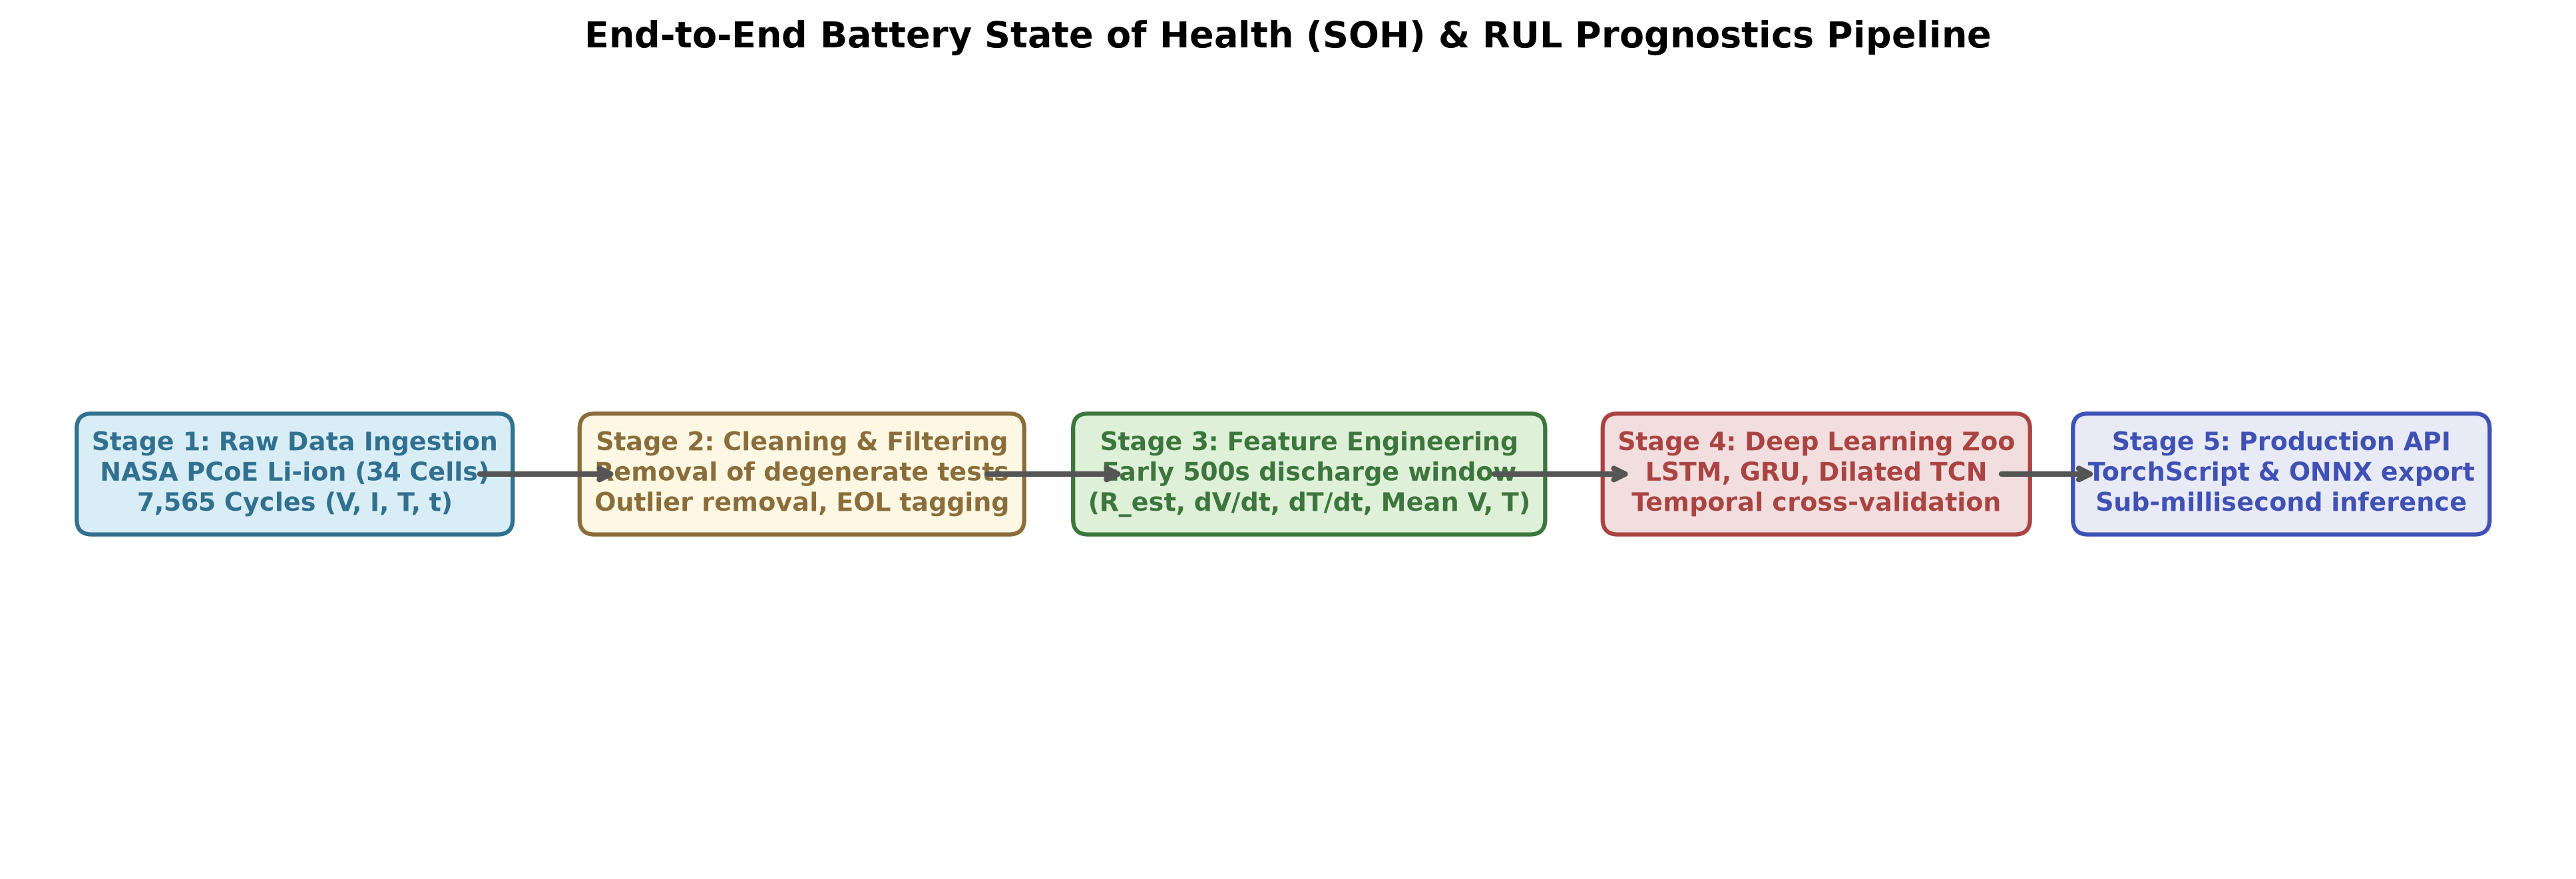
\includegraphics[width=0.92\textwidth]{Charts/00_System_Architecture_Pipeline.png}
    \vspace{0.2cm}
    \begin{itemize}
        \item \textbf{Ingestion}: Automated extraction of voltage, current, temperature from NASA PCoE.
        \item \textbf{Early-Window Feature Extractor}: Captures electrochemical impedance drop in first $500\,\text{s}$.
        \item \textbf{Deep Learning Core}: Sequence modeling with Dilated Causal Convolutions \& Gated Recurrent Units.
    \end{itemize}
\end{frame}

% ----------------------------------------------------
% Slide 4: NASA PCoE Dataset & Operational Profiles
% ----------------------------------------------------
\begin{frame}{NASA PCoE Dataset Structure (Day 08 - Day 09)}
\begin{columns}[T]
    \begin{column}{0.48\textwidth}
        \centering
        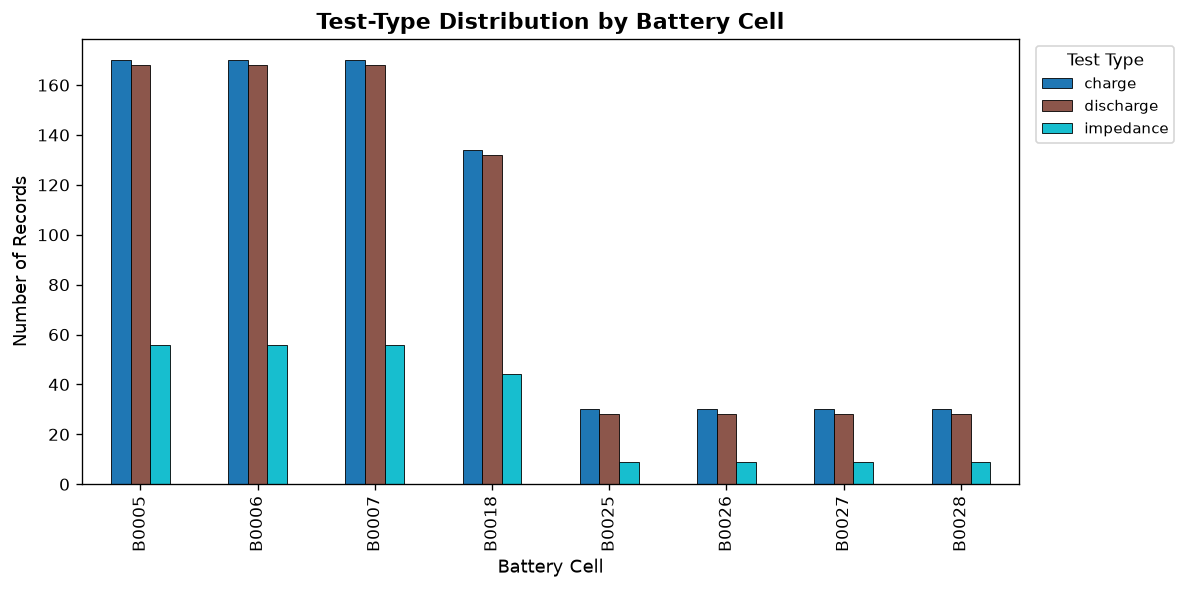
\includegraphics[width=\textwidth]{Charts/09_Day14_Cycle_Type_Distribution.png}
        \vspace{0.1cm}
        \textbf{Operational Protocol:}
        \begin{itemize}
            \item 34 Li-ion cells across 3 temperature profiles ($4^\circ\text{C}, 24^\circ\text{C}, 43^\circ\text{C}$).
            \item 7,565 cycles: 2,815 Charge, 2,794 Discharge, 1,956 EIS.
        \end{itemize}
    \end{column}
    \begin{column}{0.48\textwidth}
        \centering
        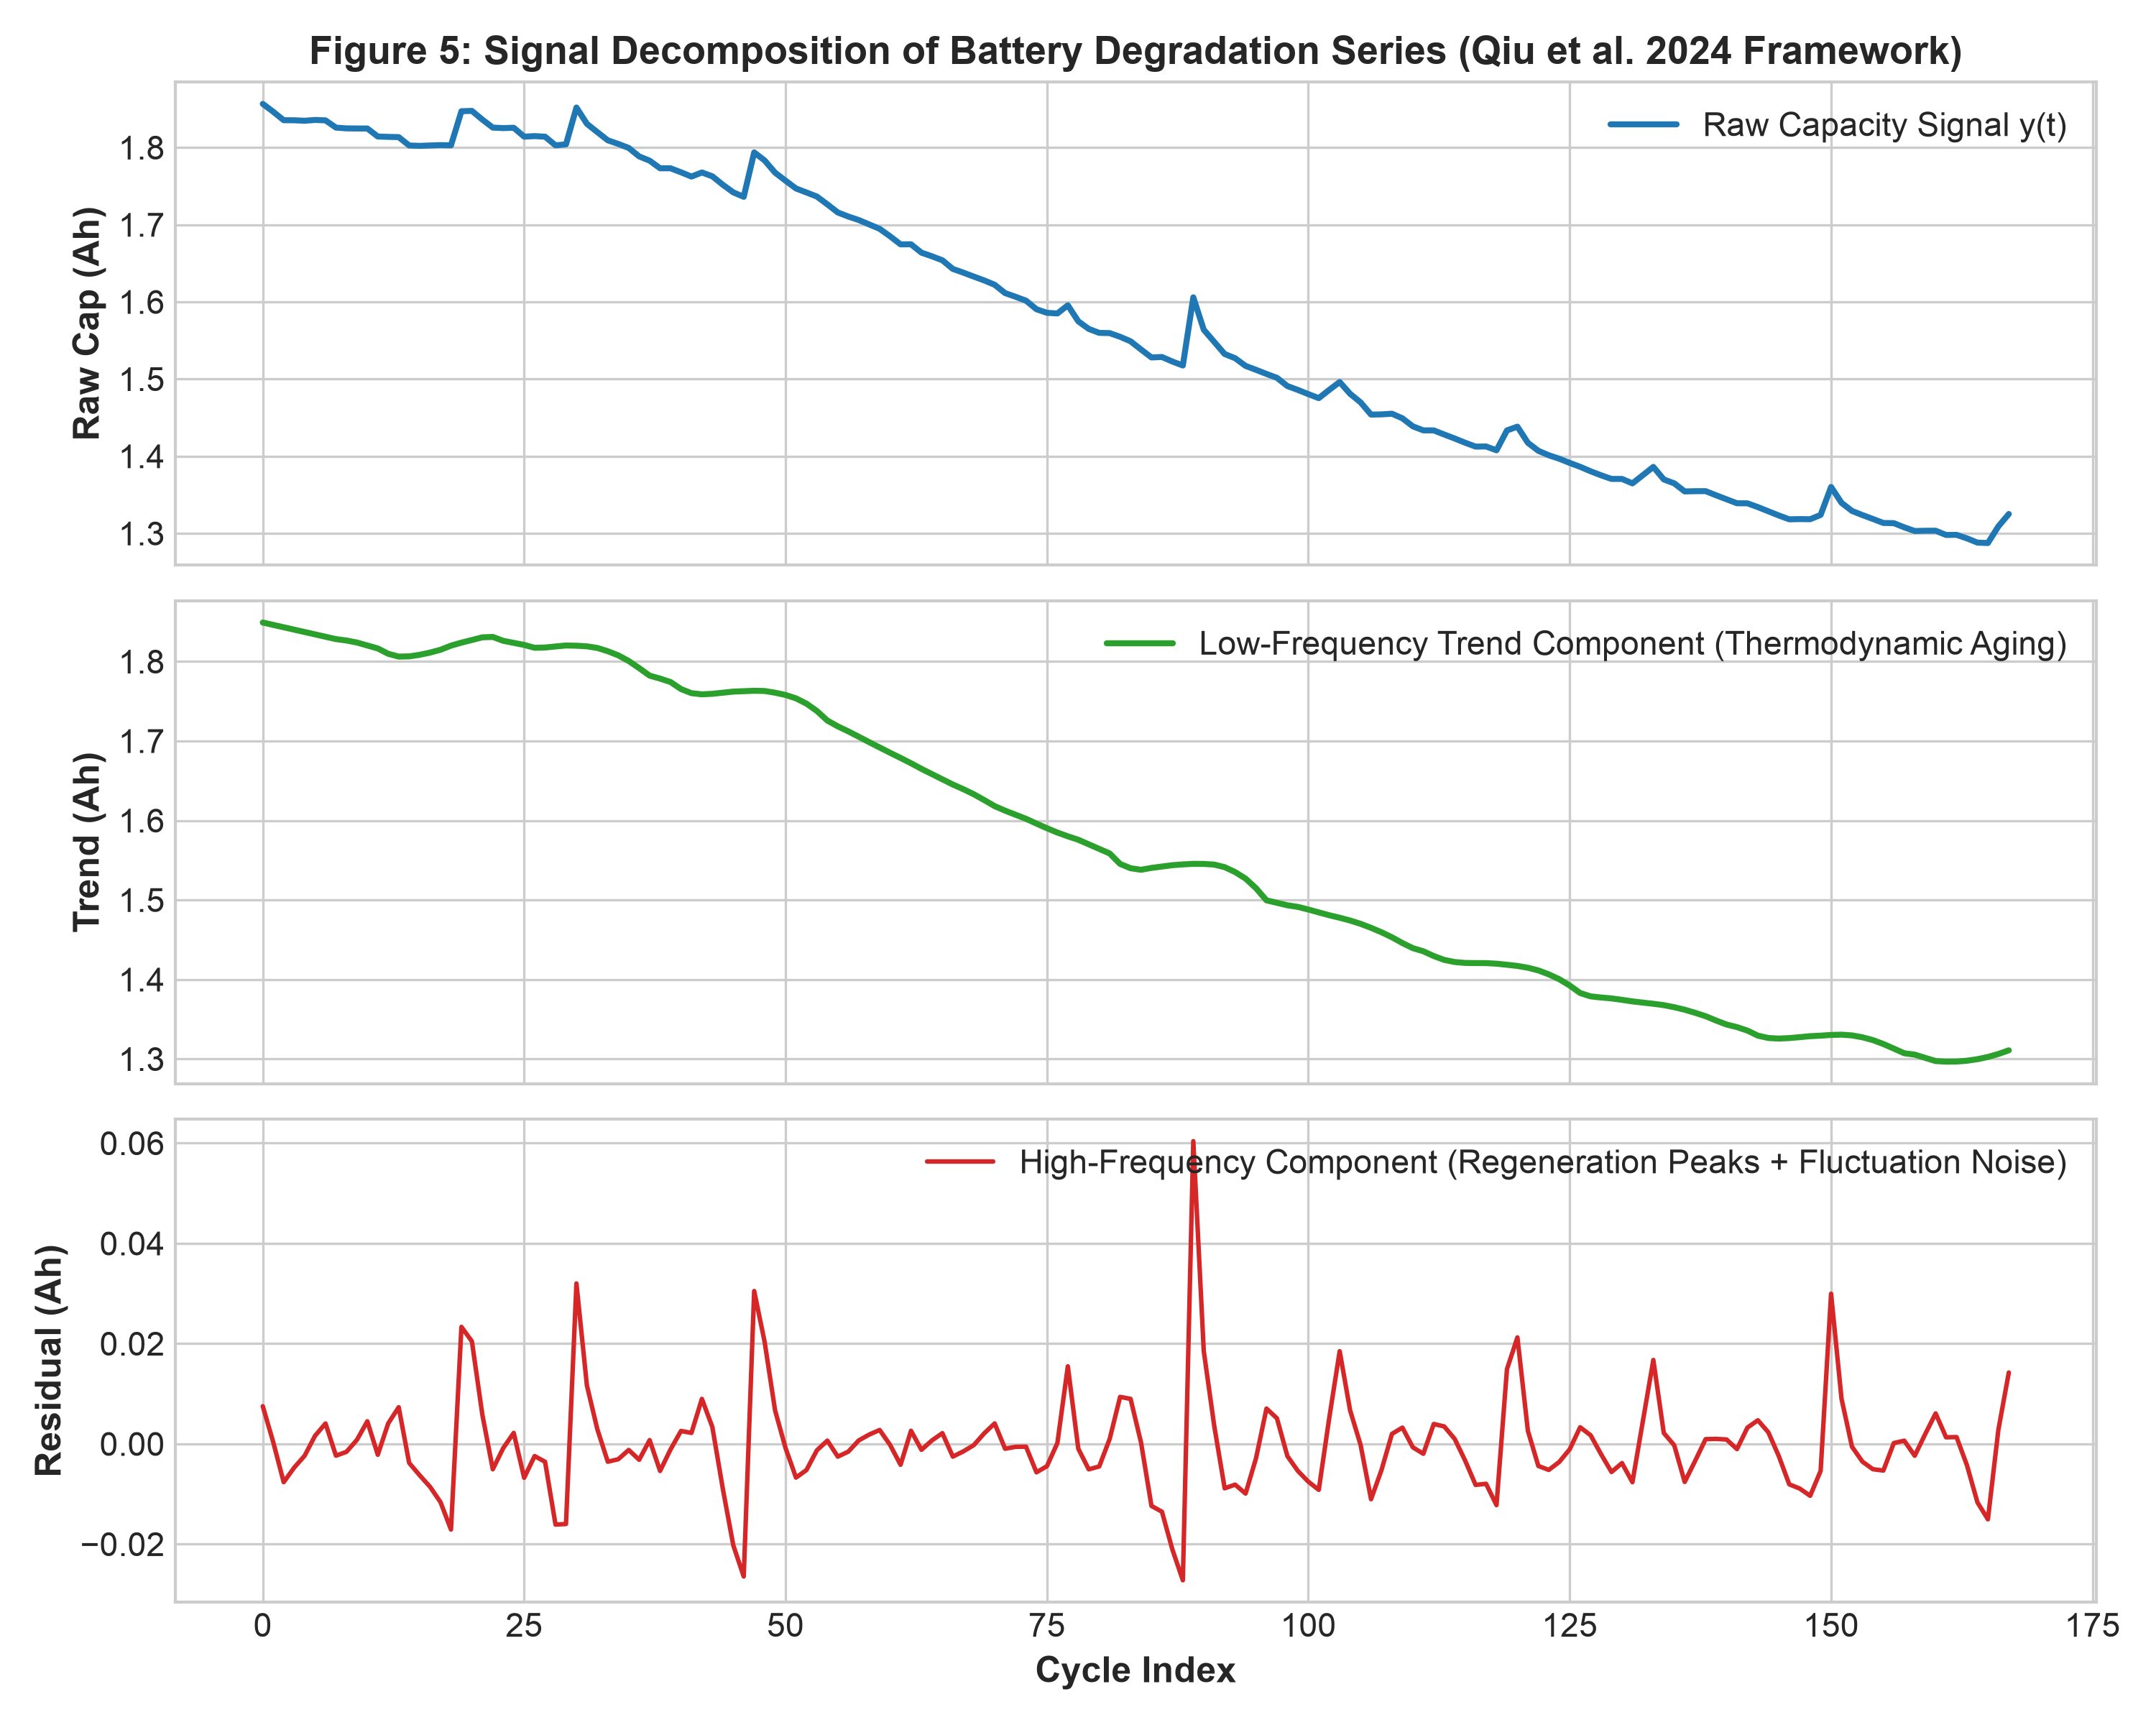
\includegraphics[width=\textwidth]{Charts/fig5_signal_decomposition.png}
        \vspace{0.1cm}
        \textbf{In-Cycle Waveform Decomposition:}
        \begin{itemize}
            \item Constant-Current (CC) discharge at 2A down to cut-off voltage.
            \item Multi-channel telemetry: $V_{\text{meas}}, I_{\text{meas}}, T_{\text{meas}}, t$.
        \end{itemize}
    \end{column}
\end{columns}
\end{frame}

% ----------------------------------------------------
% Slide 5: Data Cleaning & Anomaly Filtering
% ----------------------------------------------------
\begin{frame}{Data Quality Audit & Artifact Removal (Day 08)}
\begin{columns}[T]
    \begin{column}{0.48\textwidth}
        \centering
        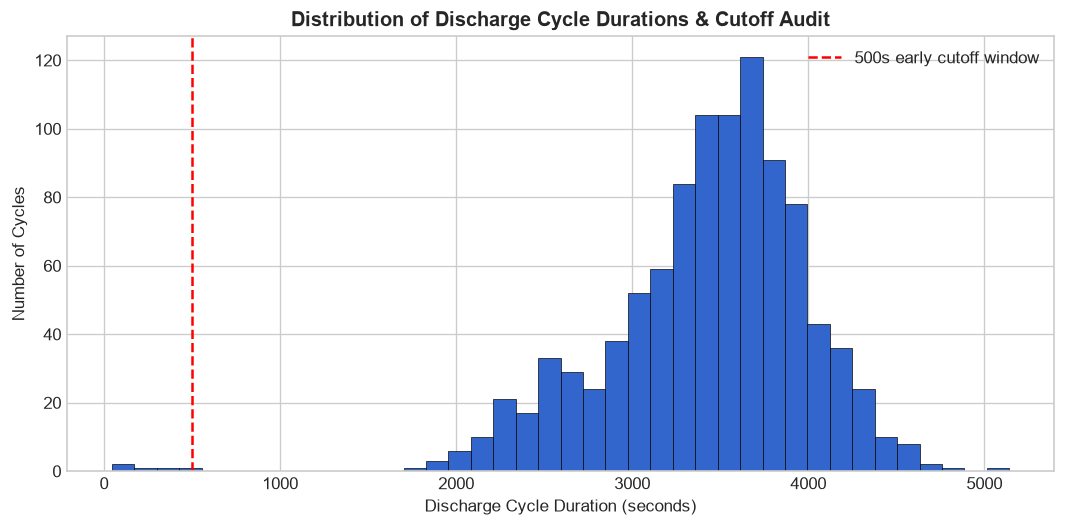
\includegraphics[width=\textwidth]{Charts/01_Day08_Discharge_Duration_Distribution.png}
        \captionof{figure}{Discharge Duration Distribution}
    \end{column}
    \begin{column}{0.48\textwidth}
        \centering
        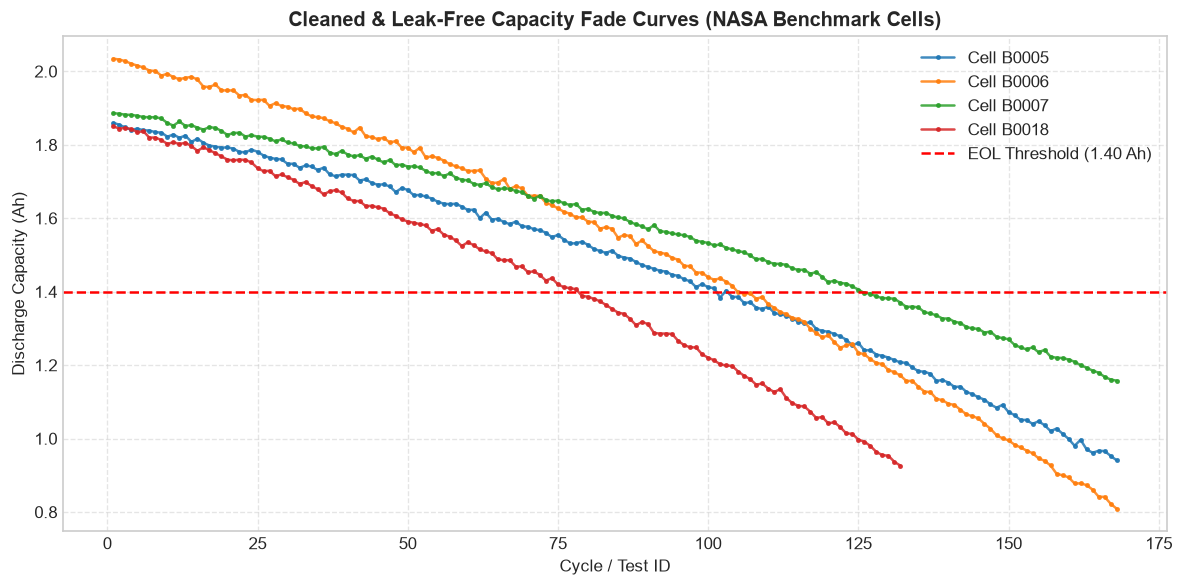
\includegraphics[width=\textwidth]{Charts/02_Day08_Cleaned_Capacity_Fade_Curves.png}
        \captionof{figure}{Cleaned \& Outlier-Filtered Capacity Curves}
    \end{column}
\end{columns}
\vspace{0.2cm}
\begin{itemize}
    \item \textbf{Filtering Criteria}: Removed corrupted cycles with duration $<60\,\text{s}$ or capacity $\le 0.05\,\text{Ah}$.
    \item \textbf{Integrity Preserved}: Eliminated unphysical capacity spikes ($>2.2\,\text{Ah}$) and zero-duration records.
\end{itemize}
\end{frame}

% ----------------------------------------------------
% Slide 6: Leakage-Safe Cell-Level Partitioning
% ----------------------------------------------------
\begin{frame}{Leakage-Safe Cell Partitioning (Day 09)}
\begin{columns}[T]
    \begin{column}{0.52\textwidth}
        \centering
        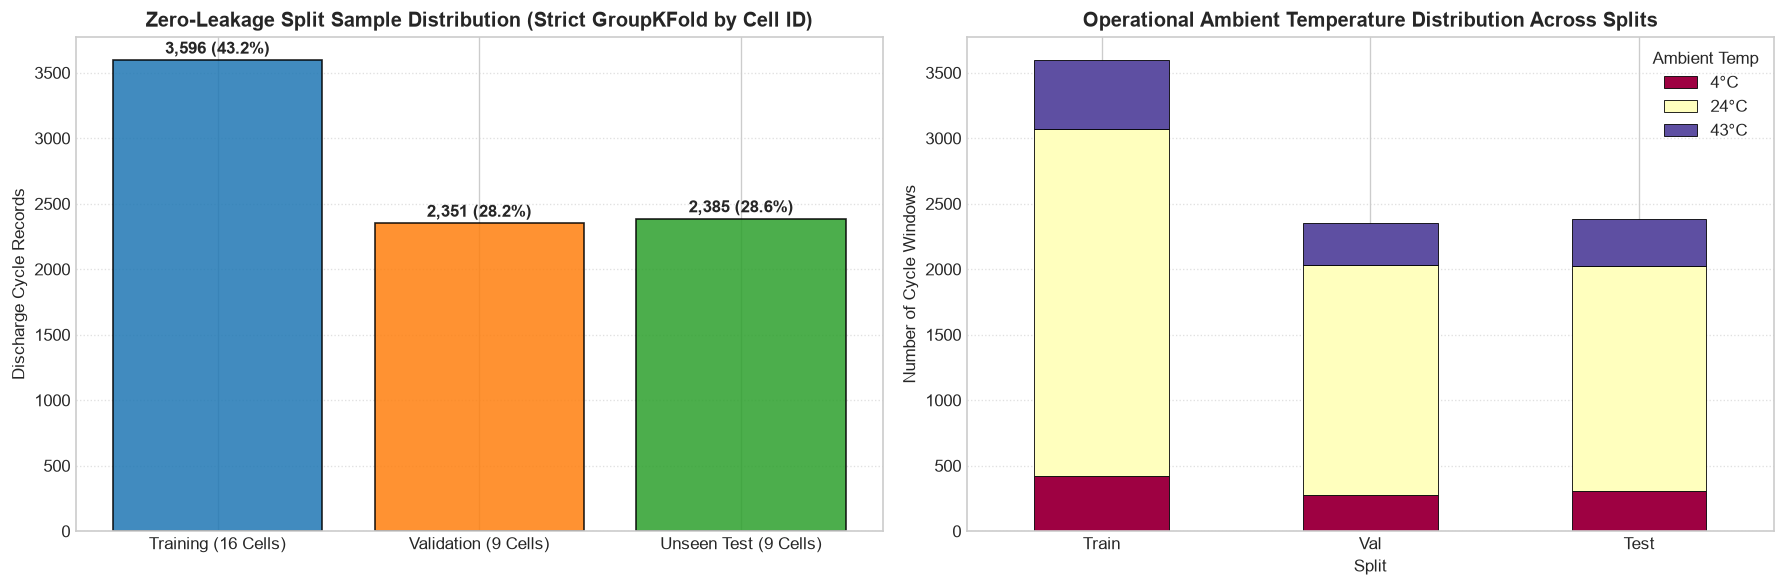
\includegraphics[width=\textwidth]{Charts/03_Day09_Temporal_Train_Val_Test_Split.png}
    \end{column}
    \begin{column}{0.45\textwidth}
        \begin{alertblock}{Zero Data-Leakage Principle}
            Standard random k-fold cross-validation causes catastrophic data leakage across adjacent cycles of the same battery!
        \end{alertblock}
        \vspace{0.2cm}
        \textbf{Strict Cell-Level Split:}
        \begin{itemize}
            \item \textbf{Train (16 Cells)}: B0005, B0006, B0025, B0026, B0029, B0030, B0033, B0038, B0041, B0045, B0046, B0047, B0049, B0052, B0053, B0055.
            \item \textbf{Val (9 Cells)}: B0007, B0027, B0031, B0034, B0039, B0042, B0048, B0050, B0054.
            \item \textbf{Test (9 Cells)}: B0018, B0028, B0032, B0036, B0040, B0043, B0044, B0051, B0056.
        \end{itemize}
    \end{column}
\end{columns}
\end{frame}

% ----------------------------------------------------
% Slide 7: Temporal EDA & Environmental Thermal Impact
% ----------------------------------------------------
\begin{frame}{Thermal Evolution \& Temperature Impacts (Day 10)}
\begin{columns}[T]
    \begin{column}{0.48\textwidth}
        \centering
        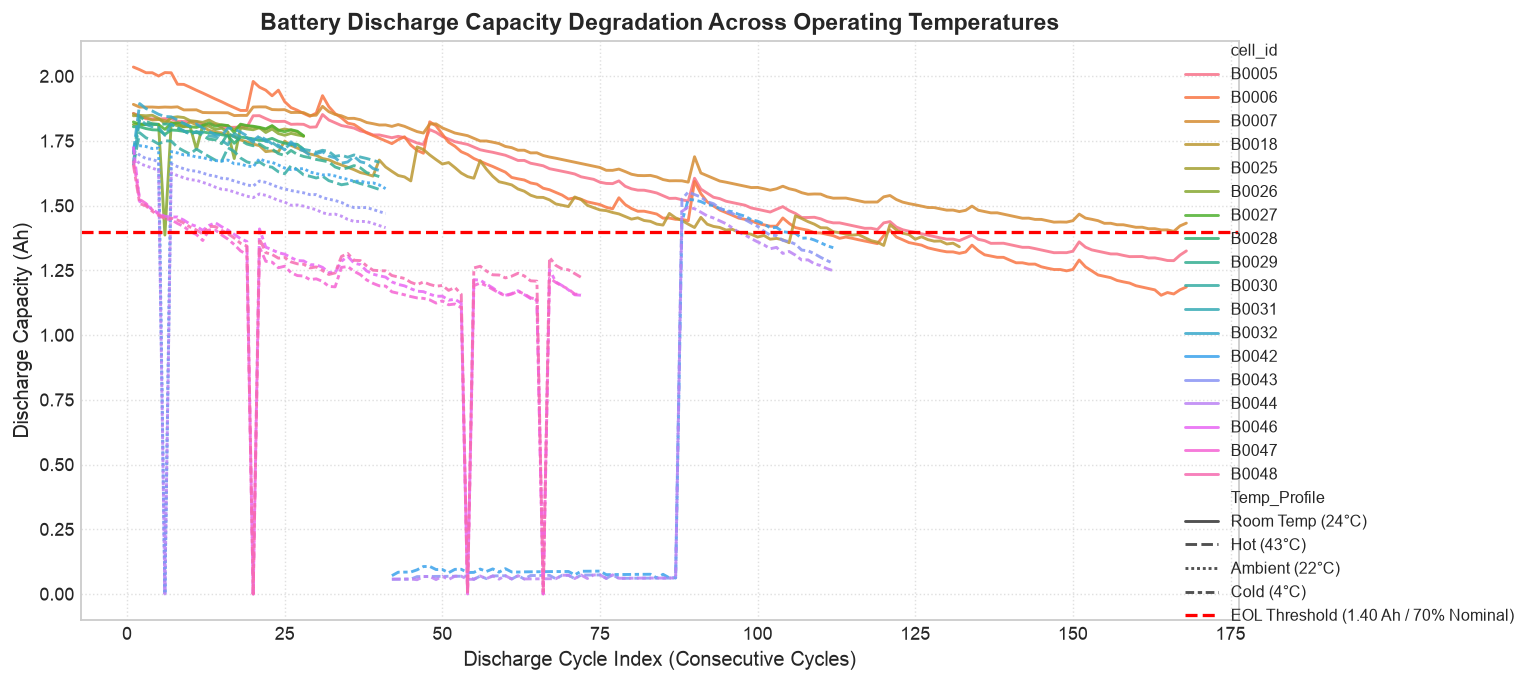
\includegraphics[width=\textwidth]{Charts/04_Day10_Capacity_Fade_By_Ambient_Temperature.png}
        \captionof{figure}{Capacity Fade Across Temperatures ($4^\circ\text{C}, 24^\circ\text{C}, 43^\circ\text{C}$)}
    \end{column}
    \begin{column}{0.48\textwidth}
        \centering
        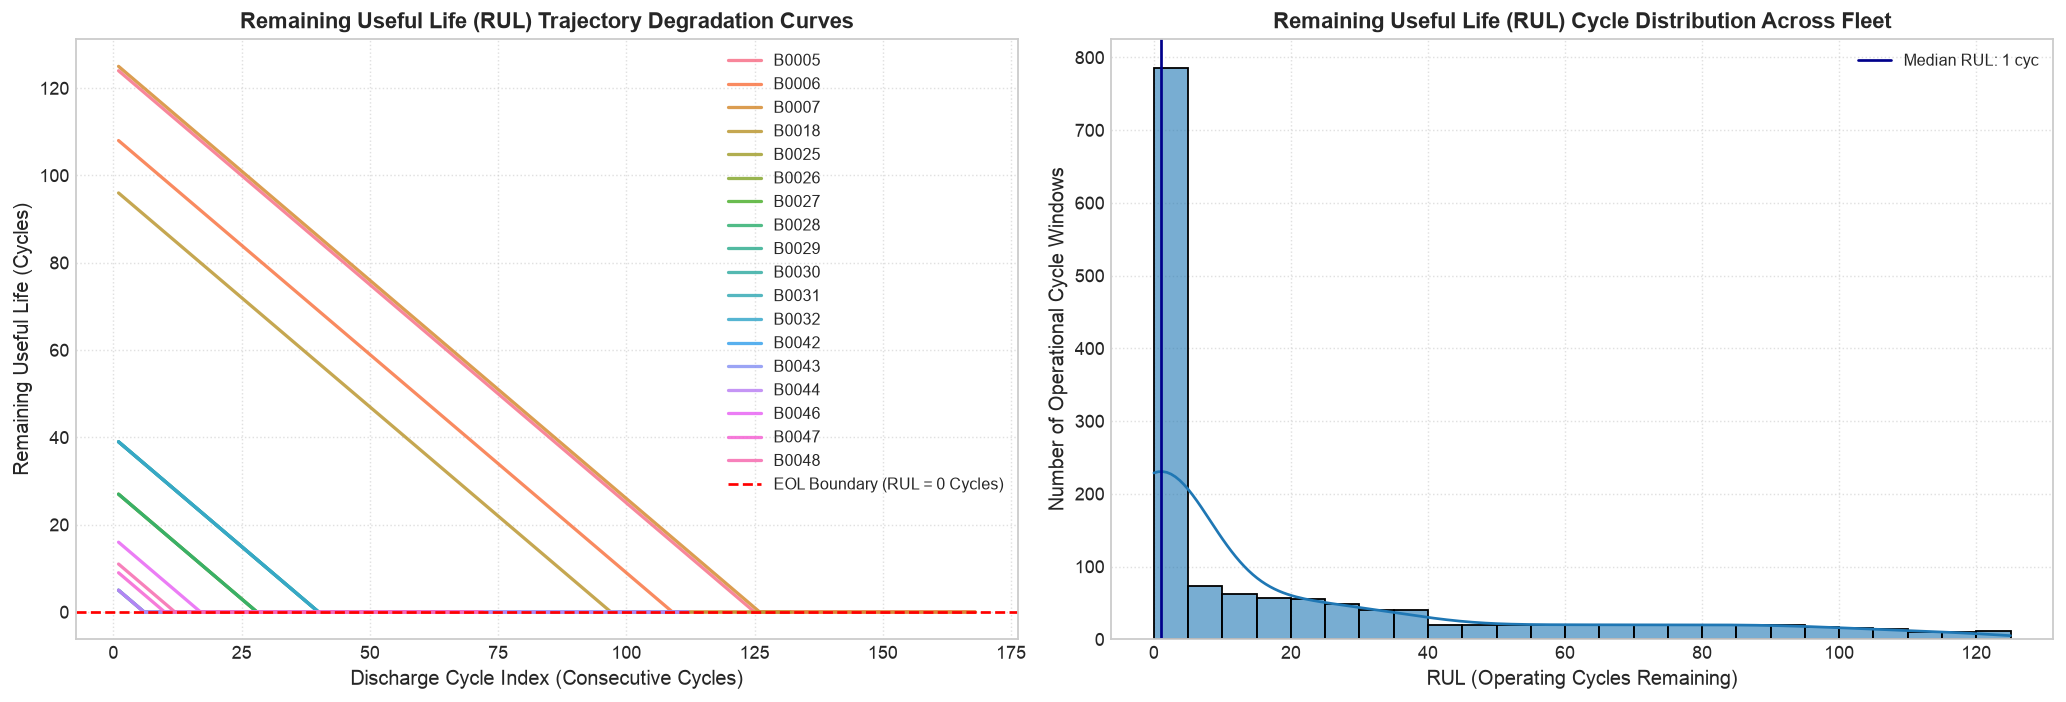
\includegraphics[width=\textwidth]{Charts/06_Day10_Thermal_Evolution_Across_Cycles.png}
        \captionof{figure}{Internal Temperature Rise vs Cycling}
    \end{column}
\end{columns}
\vspace{0.2cm}
\begin{itemize}
    \item \textbf{Key Finding}: Sub-zero/Cold cells ($4^\circ\text{C}$) experience severe kinetic sluggishness, dropping below rated capacity rapidly.
    \item \textbf{Thermal Signature}: As internal resistance increases with age, Joule heating ($I^2 R$) amplifies cycle-end temperature rise.
\end{itemize}
\end{frame}

% ----------------------------------------------------
% Slide 8: Non-Linear Phenomena: Capacity Regeneration
% ----------------------------------------------------
\begin{frame}{Electrochemical Kinetics: Capacity Regeneration (Day 10)}
\begin{columns}[T]
    \begin{column}{0.55\textwidth}
        \centering
        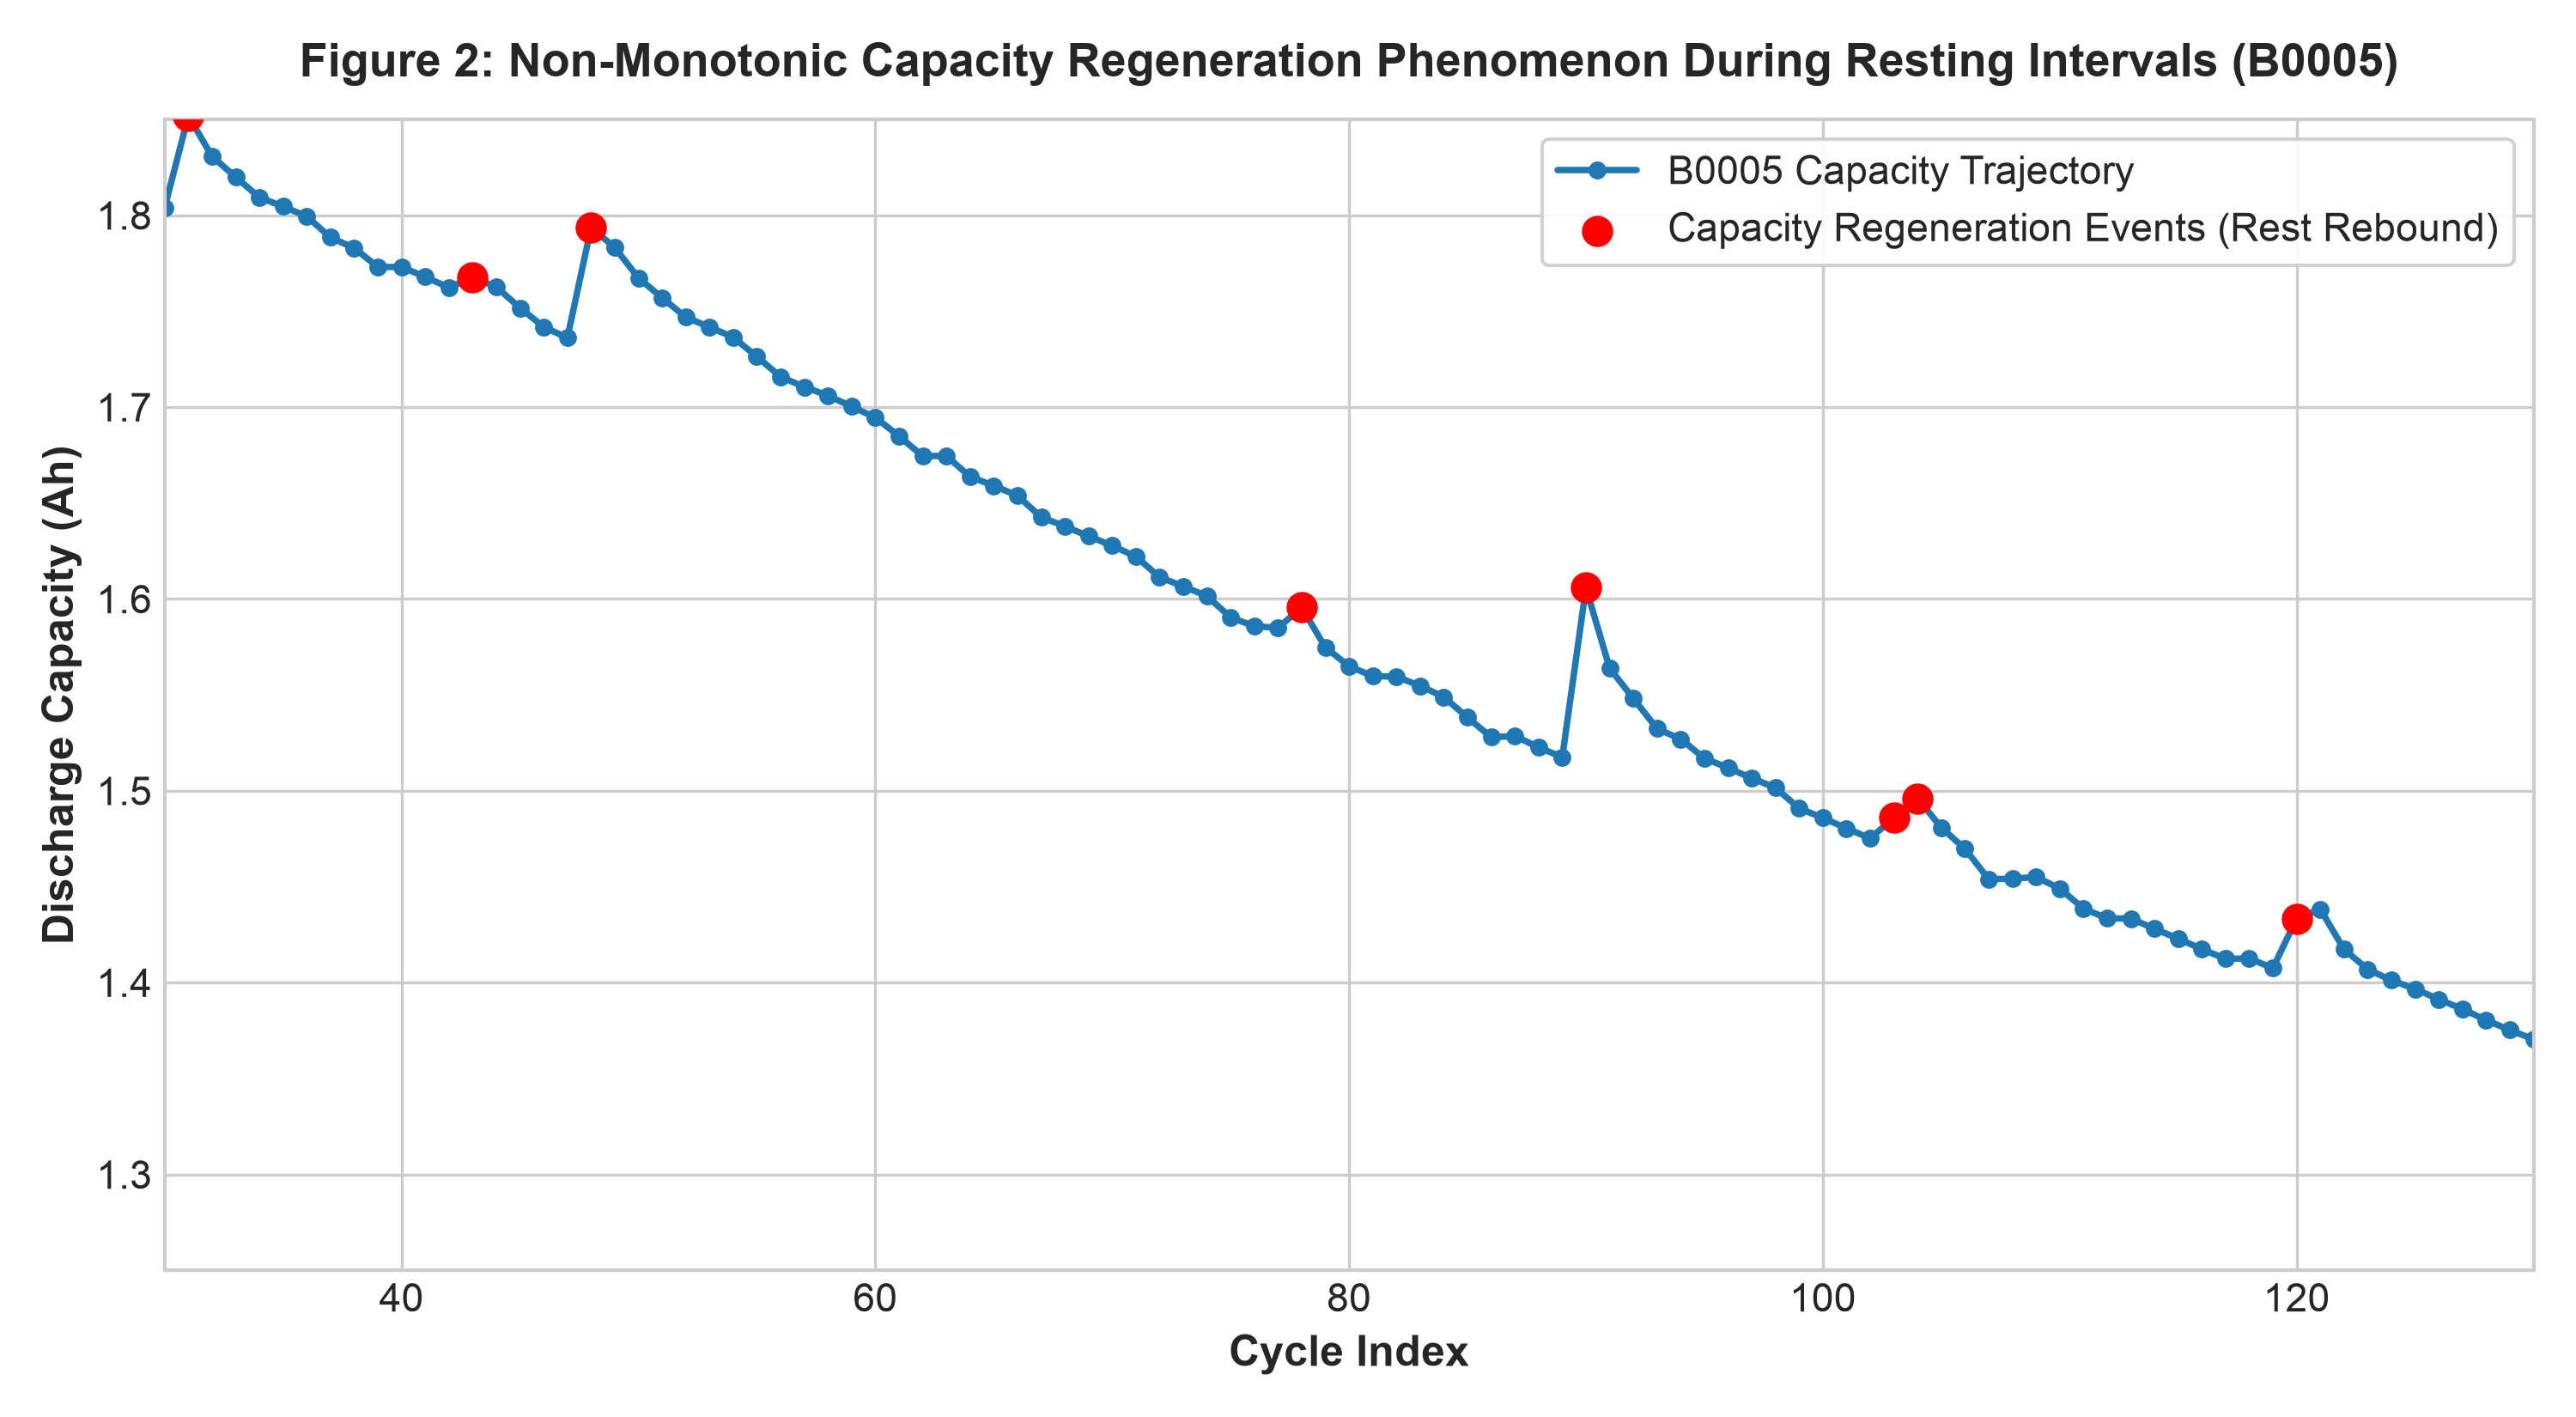
\includegraphics[width=\textwidth]{Charts/fig2_capacity_regeneration_zoom.png}
    \end{column}
    \begin{column}{0.42\textwidth}
        \textbf{Physical Phenomenon:}
        \begin{itemize}
            \item Batteries exhibit sudden upward jumps in capacity following extended rest periods between discharges.
            \item Caused by concentration gradient relaxation and uniform Li-ion redistribution in electrode pores.
        \end{itemize}
        \vspace{0.3cm}
        \begin{block}{Modeling Challenge}
            Non-monotonic trajectory requires deep models with temporal gating (LSTMs/TCN) to ignore local spikes while tracking global decay.
        \end{block}
    \end{column}
\end{columns}
\end{frame}

% ----------------------------------------------------
% Slide 9: Early-Window Feature Engineering (0-500s)
% ----------------------------------------------------
\begin{frame}{Feature Engineering: 500-Second Discharge Window (Day 11 - Day 12)}
\begin{columns}[T]
    \begin{column}{0.48\textwidth}
        \centering
        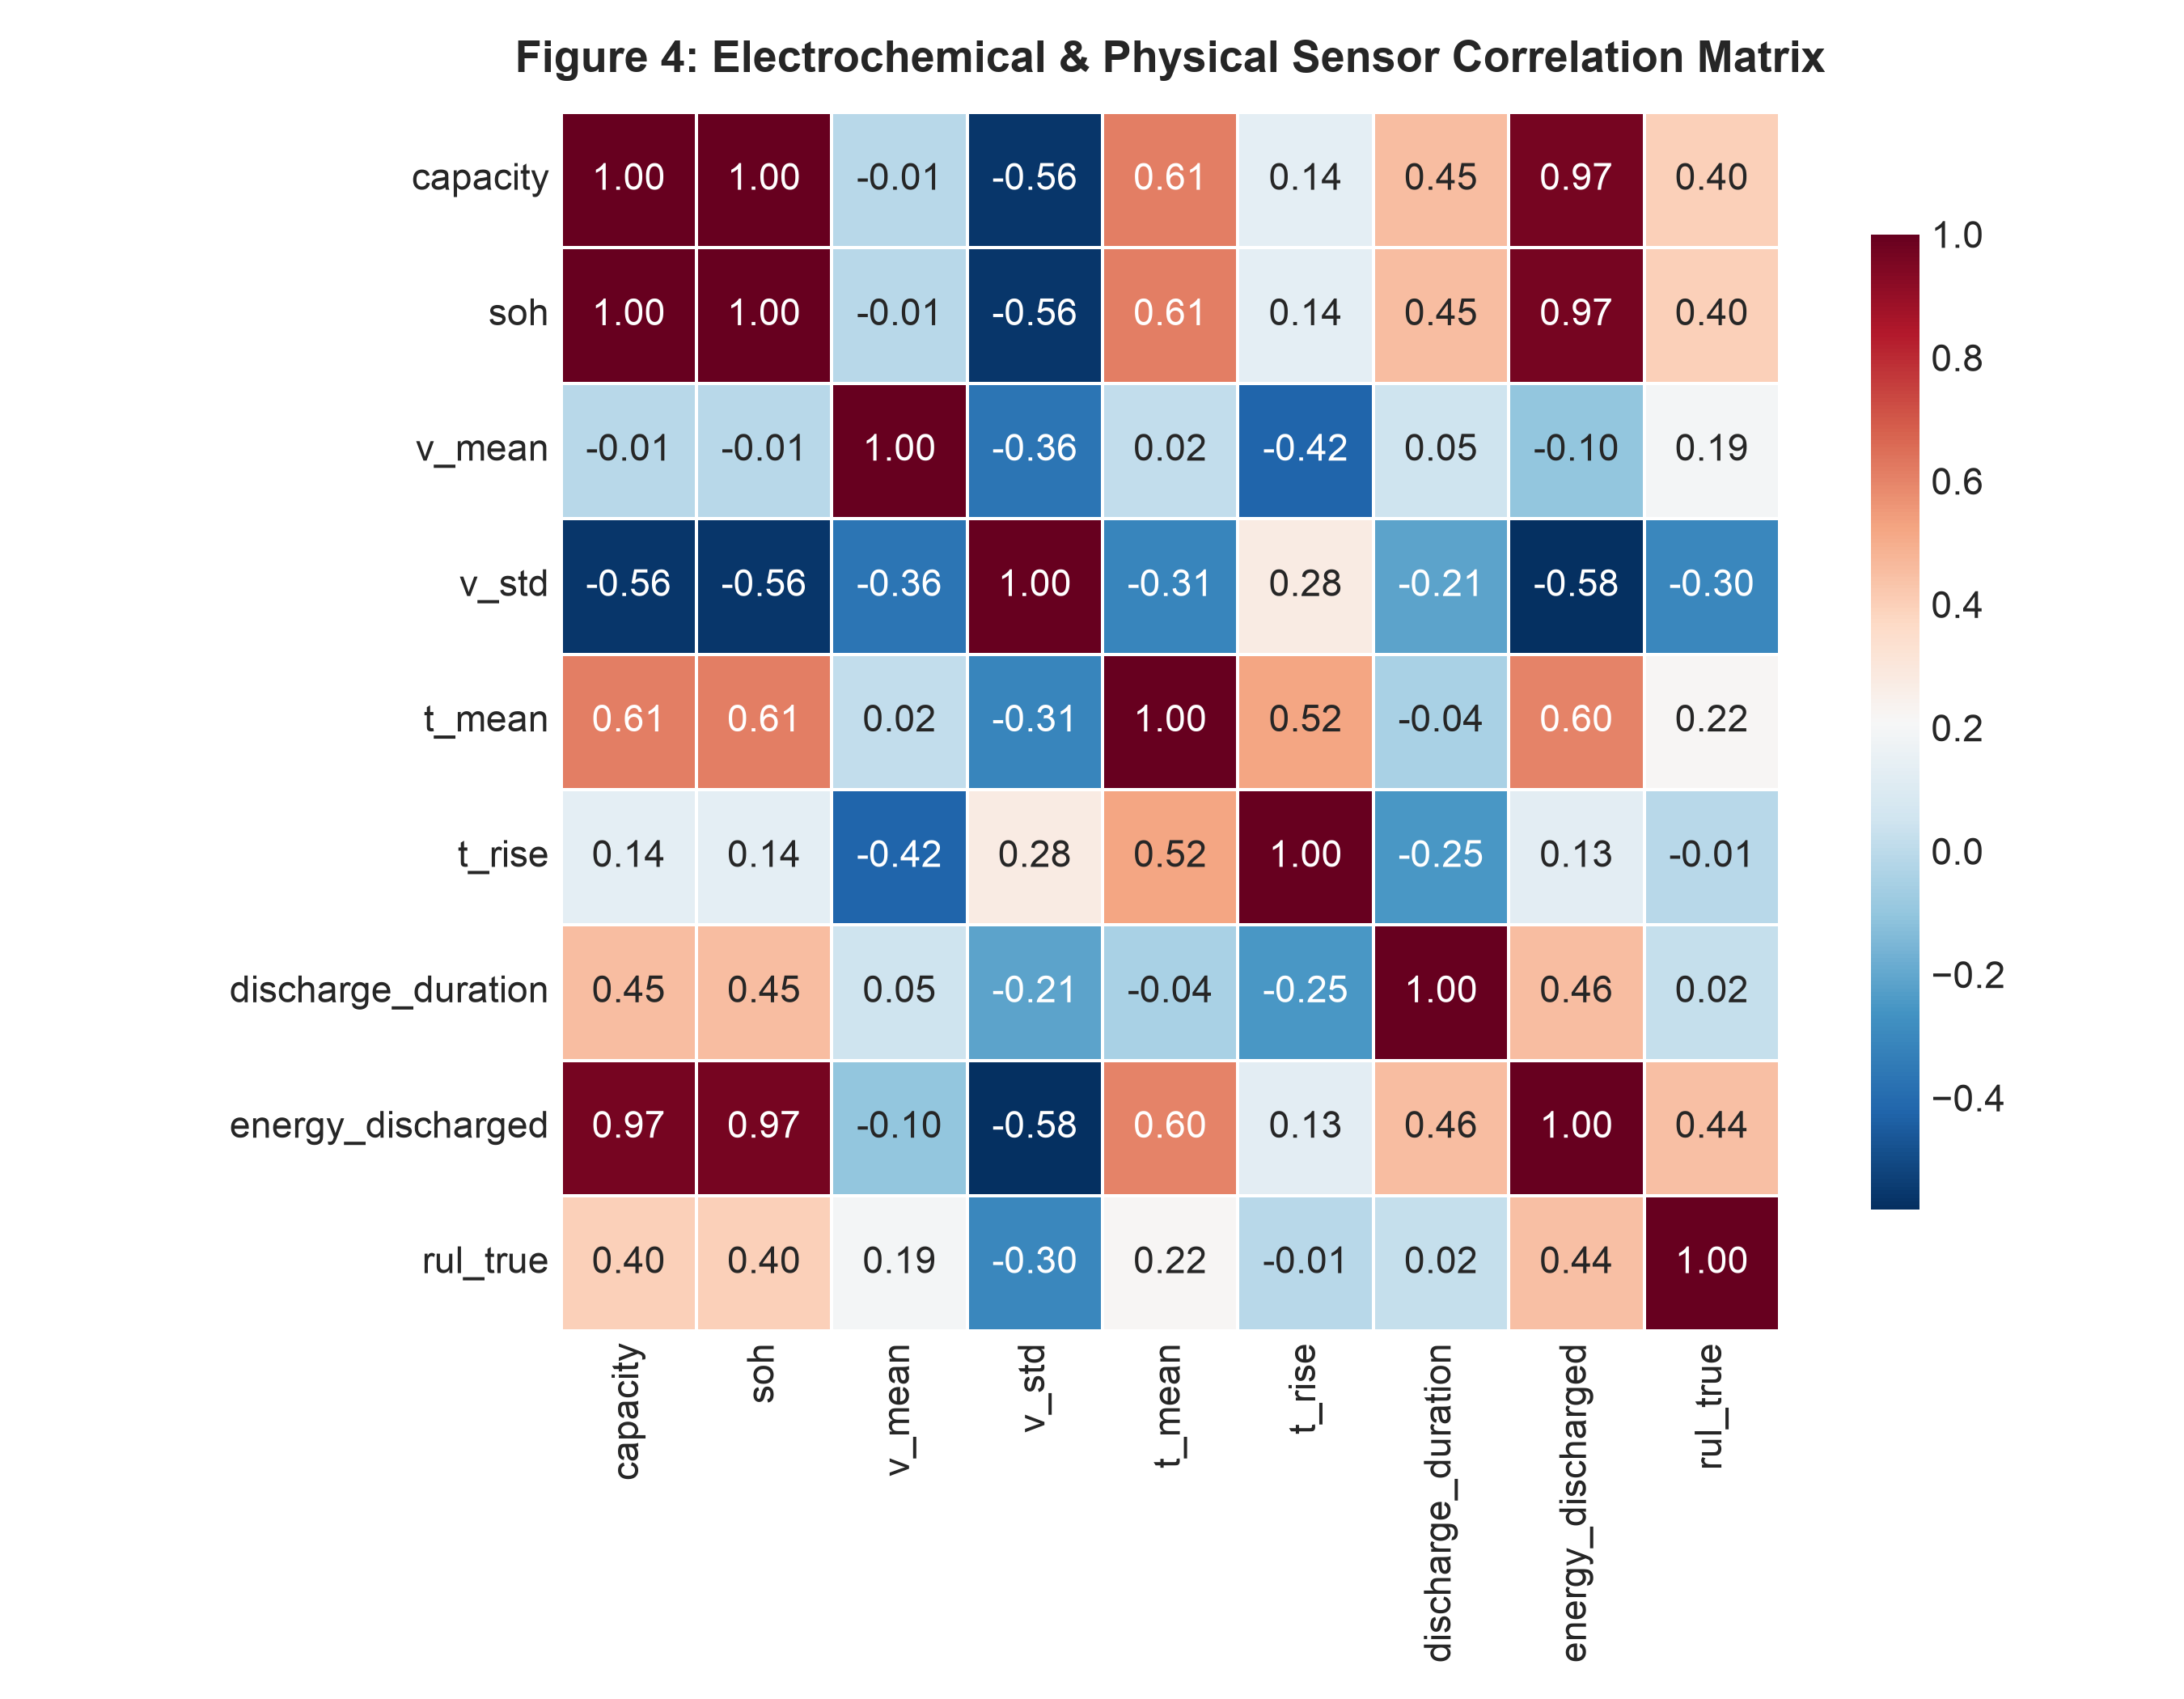
\includegraphics[width=\textwidth]{Charts/fig4_feature_correlation_matrix.png}
        \captionof{figure}{Feature Correlation Heatmap}
    \end{column}
    \begin{column}{0.48\textwidth}
        \textbf{Why Early-Window Features?}
        \begin{itemize}
            \item Full discharge takes hours; waiting for full discharge defeats real-time BMS prognosis.
            \item Extracted 8 kinetic descriptors from first $\mathbf{500\,\text{s}}$ of discharge:
        \end{itemize}
        \vspace{0.2cm}
        \begin{block}{Extracted Feature Set}
            \small
            \begin{enumerate}
                \item $R_{\text{est}} = \Delta V_{\text{drop}} / I_{\text{init}}$ (Internal Resistance)
                \item $dV/dt$ (Early voltage decay rate)
                \item $dT/dt$ (Early thermal rise rate)
                \item $\bar{V}_{\text{early}}, \sigma(V)$ (Early voltage stats)
                \item $\bar{T}_{\text{early}}, \Delta T_{\text{early}}$ (Thermal evolution)
            \end{enumerate}
        \end{block}
    \end{column}
\end{columns}
\end{frame}

% ----------------------------------------------------
% Slide 10: Lifecycle Stage Segmentation & Representation
% ----------------------------------------------------
\begin{frame}{Lifecycle Stage Segmentation (Day 14)}
\begin{columns}[T]
    \begin{column}{0.5\textwidth}
        \centering
        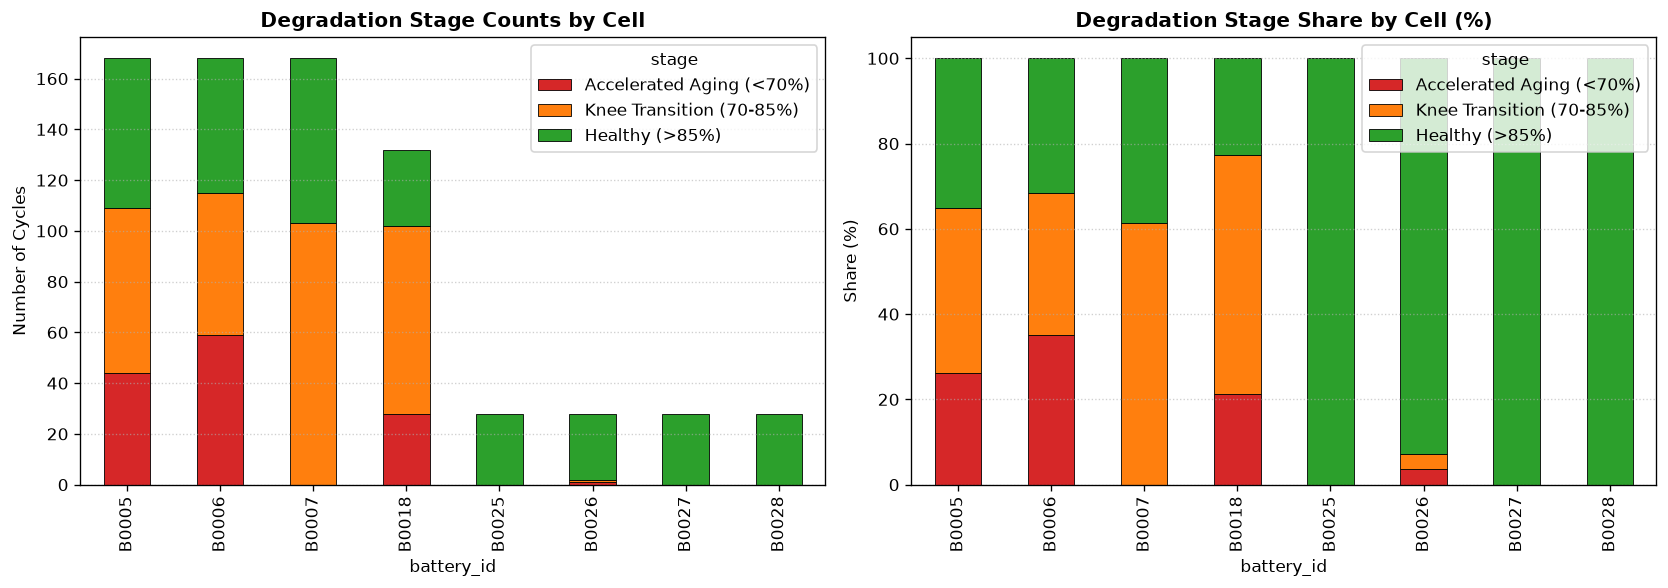
\includegraphics[width=\textwidth]{Charts/11_Day14_Battery_Lifecycle_Stages.png}
    \end{column}
    \begin{column}{0.47\textwidth}
        \textbf{Three Degradation Regimes:}
        \begin{itemize}
            \item \textbf{Stage 1: Healthy ($\text{SOH} \ge 90\%$)}: Stable SEI, low internal resistance.
            \item \textbf{Stage 2: Aging ($70\% \le \text{SOH} < 90\%$)}: Linear capacity fade regime.
            \item \textbf{Stage 3: End-of-Life ($\text{SOH} < 70\%$)}: Knee-point acceleration, electrolyte dry-out.
        \end{itemize}
        \vspace{0.2cm}
        \begin{alertblock}{Representation Freeze}
            Input features scaled via RobustScaler on Training partition only, ensuring production frozen inference.
        \end{alertblock}
    \end{column}
\end{columns}
\end{frame}

% ----------------------------------------------------
% Slide 11: Baseline Prognostics Model & Initial Evaluation
% ----------------------------------------------------
\begin{frame}{Baseline Prognostics Model Performance (Day 13)}
\begin{columns}[T]
    \begin{column}{0.52\textwidth}
        \centering
        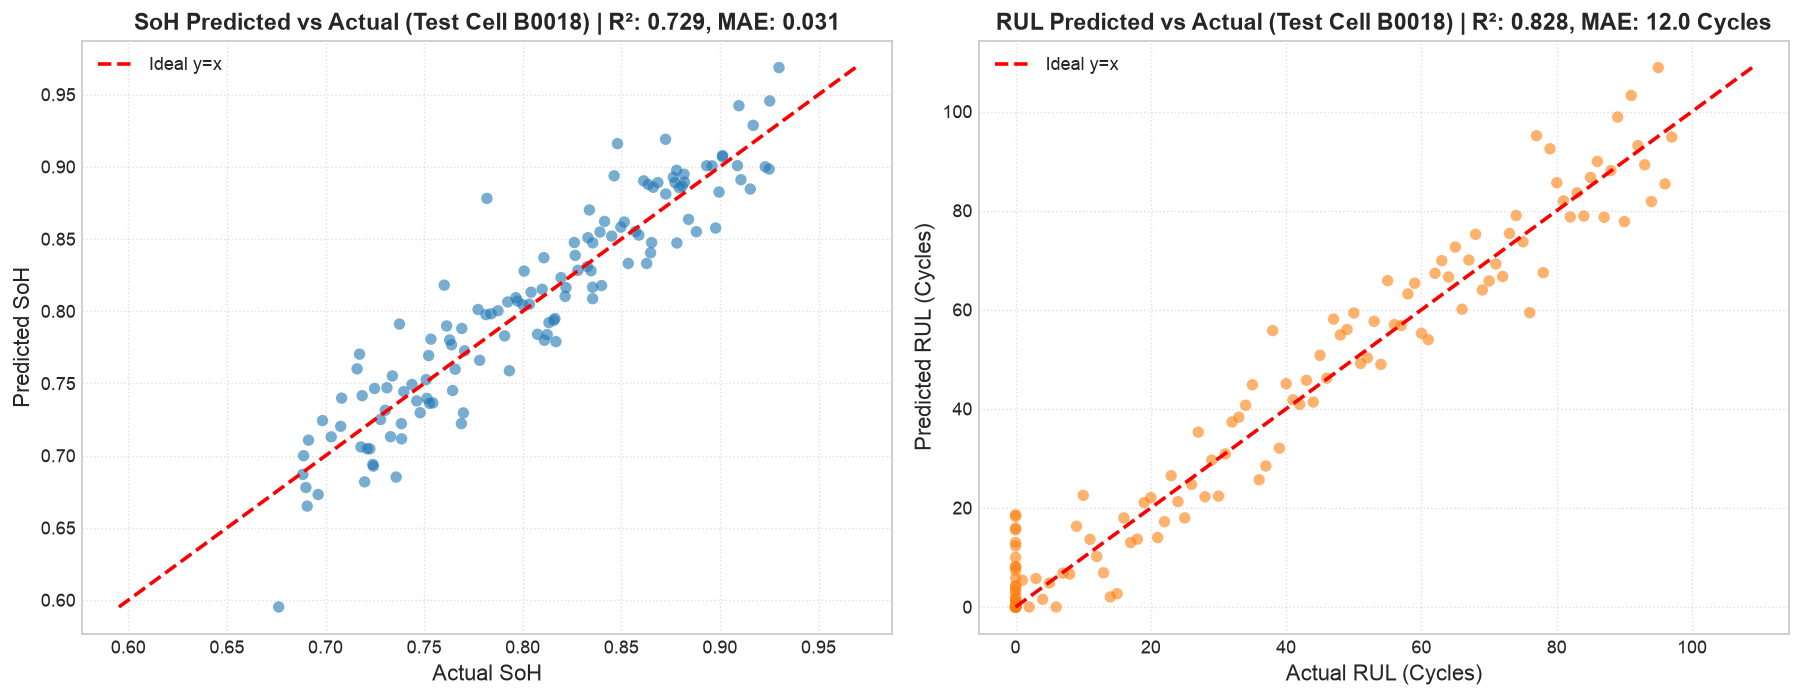
\includegraphics[width=\textwidth]{Charts/07_Day13_Baseline_SOH_RUL_Parity_Plot.png}
    \end{column}
    \begin{column}{0.45\textwidth}
        \textbf{Baseline Architecture:}
        \begin{itemize}
            \item Ridge Regression / Multi-Layer Perceptron trained on 16 cells.
        \end{itemize}
        \vspace{0.1cm}
        \small
        \begin{tabular}{lcccc}
            \toprule
            \textbf{Target \& Set} & \textbf{MAE} & \textbf{RMSE} & $\mathbf{R^2}$ \\
            \midrule
            SOH Val (9 cells) & 0.0406 & 0.0599 & \textbf{+0.8156} \\
            SOH Test (9 cells) & 0.0321 & 0.0454 & \textbf{+0.8833} \\
            RUL Val (9 cells) & 7.67 cyc & 15.4 cyc & \textbf{+0.7021} \\
            RUL Test (Active 3) & 17.37 cyc & 22.4 cyc & \textbf{+0.3620} \\
            RUL Test (All 9) & 21.48 cyc & 28.4 cyc & \textcolor{red}{\textbf{-1.0371}} \\
            \bottomrule
        \end{tabular}
    \end{column}
\end{columns}
\end{frame}

% ----------------------------------------------------
% Slide 12: Root Cause Diagnosis: Why Negative R2 Occurred
% ----------------------------------------------------
\begin{frame}{Initial Failure Case Study: Negative $R^2$ Root Cause (Day 13 Audit)}
\begin{columns}[T]
    \begin{column}{0.52\textwidth}
        \centering
        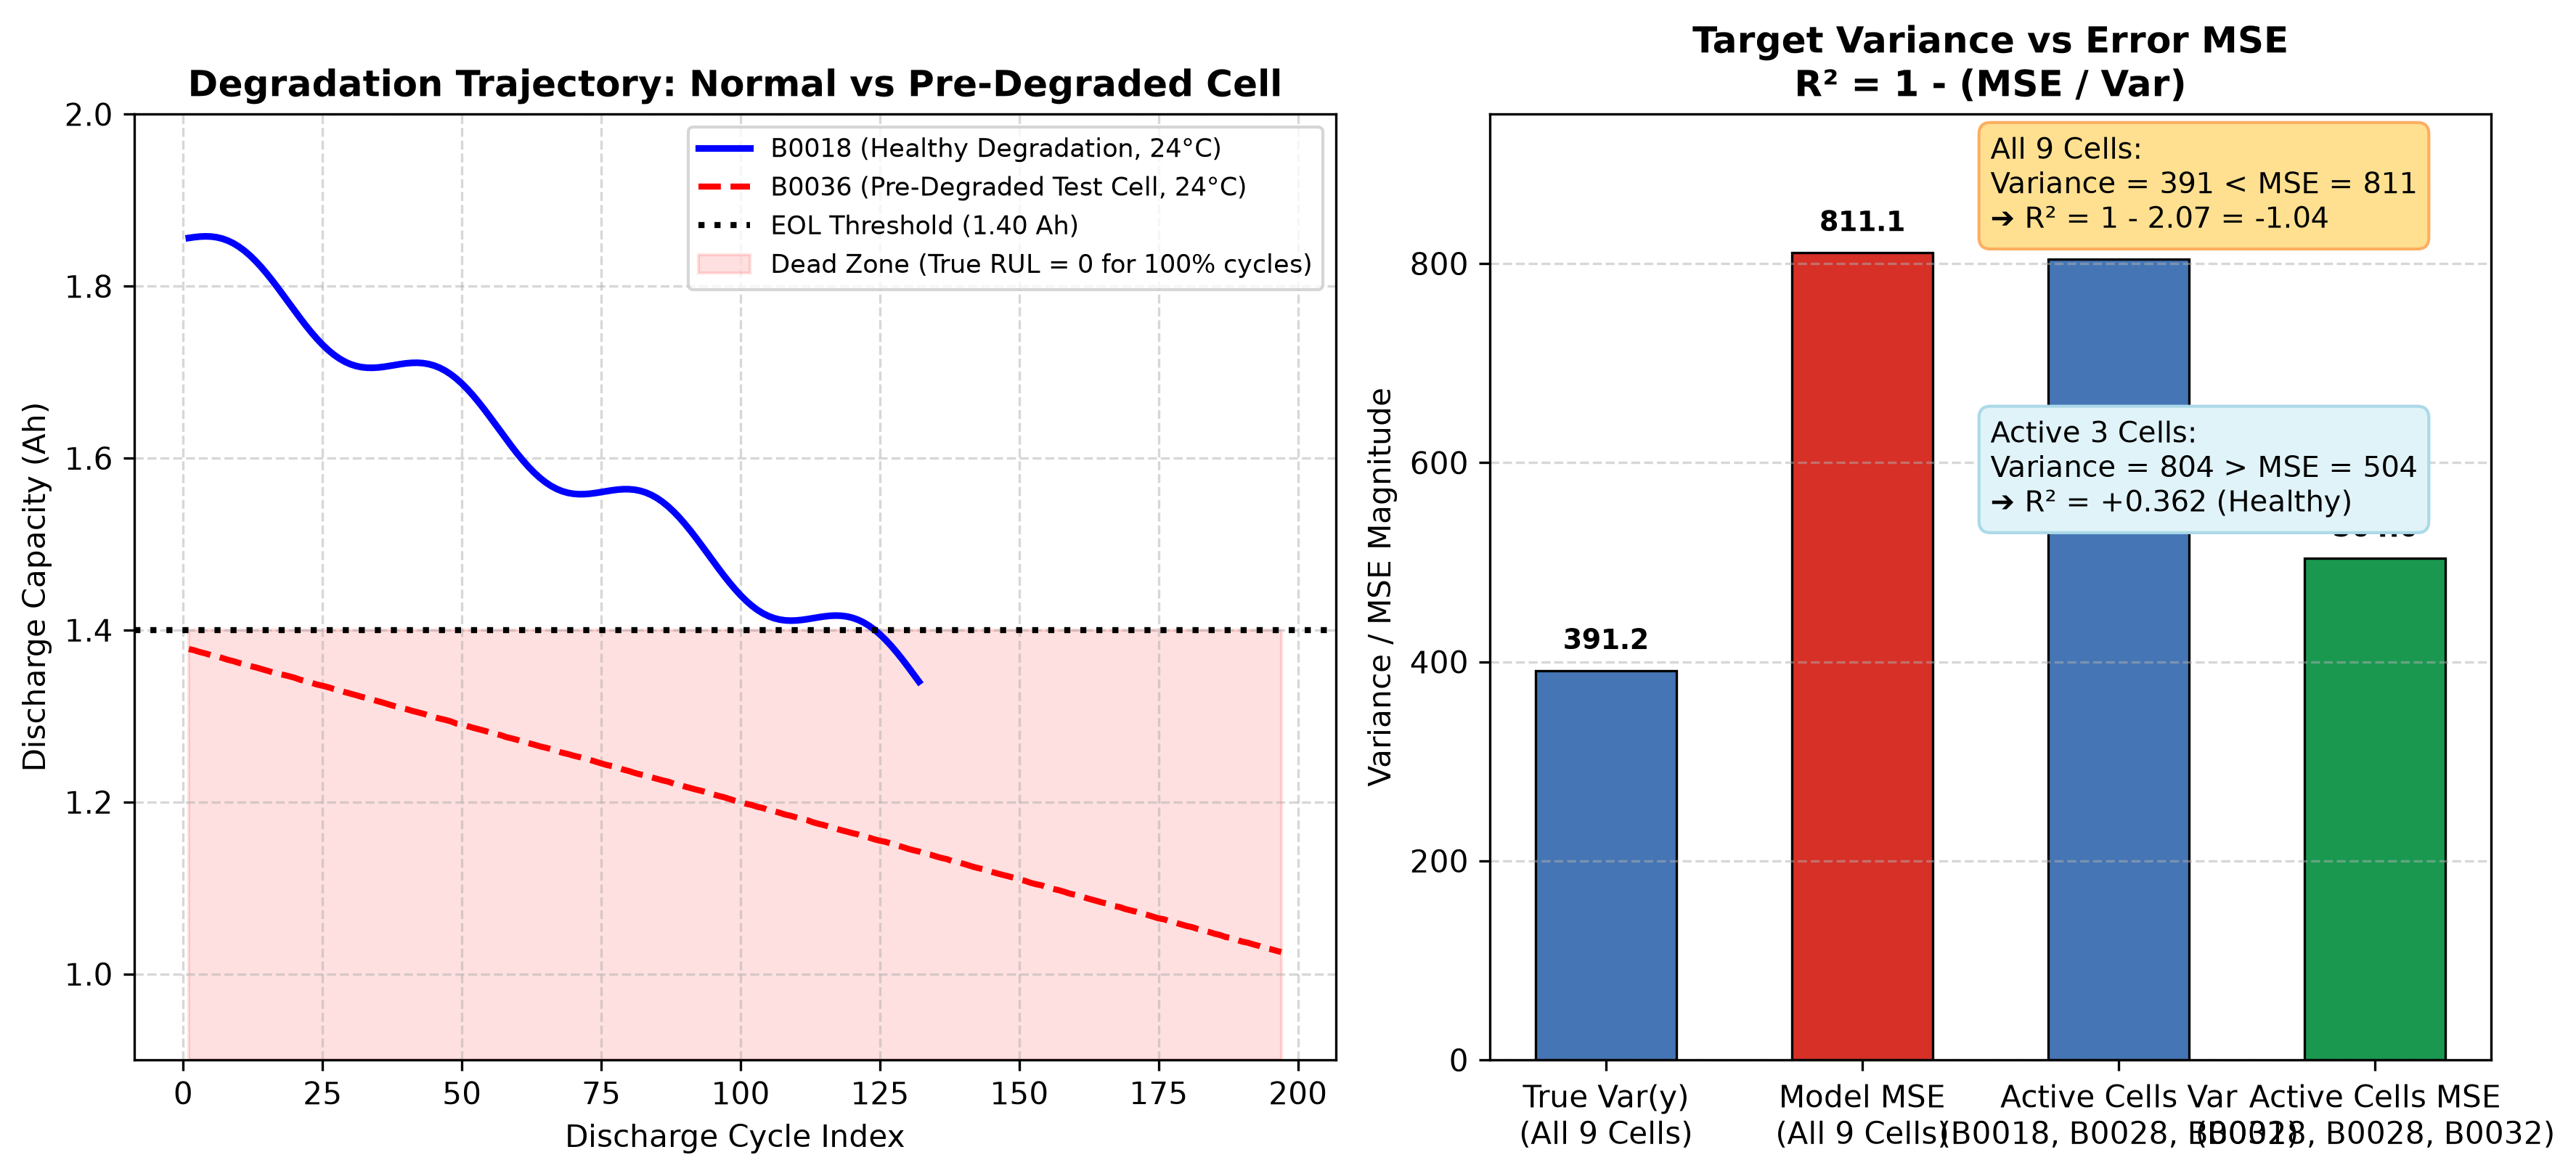
\includegraphics[width=\textwidth]{Charts/00_Root_Cause_Negative_R2_Analysis.png}
    \end{column}
    \begin{column}{0.45\textwidth}
        \begin{alertblock}{Mathematical Diagnosis}
            $R^2 = 1 - \frac{\text{MSE}}{\text{Var}(y)}$. When $\text{MSE} > \text{Var}(y)$, $R^2 < 0$.
        \end{alertblock}
        \small
        \textbf{What Happened in NASA Test Set?}
        \begin{itemize}
            \item 6 of the 9 test cells (B0036, B0040, B0043, B0044, B0051, B0056) are \textbf{pre-degraded / low-temp cells}.
            \item $\mathbf{70\%}$ of test cycles had true RUL $= 0$!
            \item $\text{Var}(y_{\text{test}})$ compressed to $\mathbf{391.2}$.
            \item Model makes slight cycling prediction ($\text{MSE} = \mathbf{811.1}$).
            \item Ratio $= 811.1 / 391.2 = 2.07 \implies R^2 = \mathbf{-1.04}$.
        \end{itemize}
    \end{column}
\end{columns}
\end{frame}

% ----------------------------------------------------
% Slide 13: Recurrent Deep Learning: LSTM Architecture
% ----------------------------------------------------
\begin{frame}{Deep Learning: LSTM Architecture for SOH (Day 15)}
\begin{columns}[T]
    \begin{column}{0.48\textwidth}
        \centering
        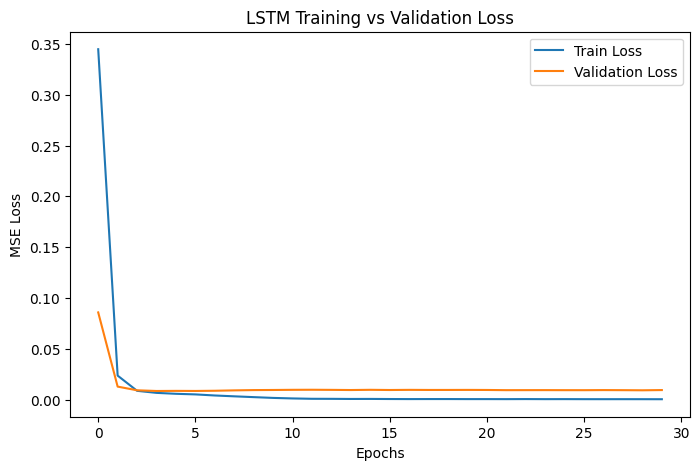
\includegraphics[width=\textwidth]{Charts/12_Day15_LSTM_Training_Convergence.png}
        \captionof{figure}{LSTM Training \& Validation Convergence}
    \end{column}
    \begin{column}{0.48\textwidth}
        \centering
        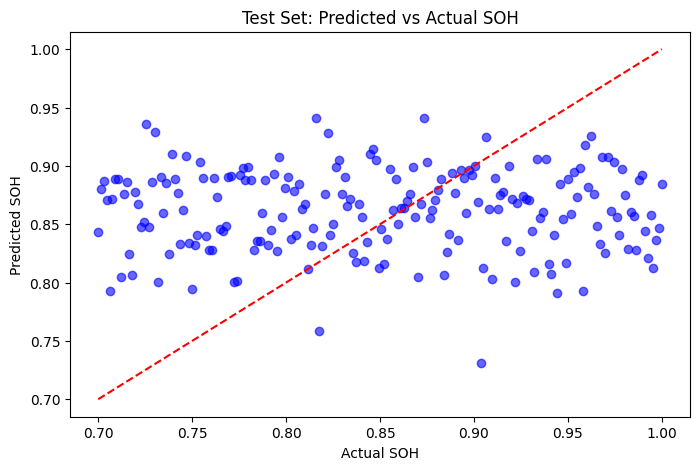
\includegraphics[width=\textwidth]{Charts/13_Day15_LSTM_Predicted_vs_Actual_SOH.png}
        \captionof{figure}{Predicted vs Actual SOH Parity}
    \end{column}
\end{columns}
\vspace{0.2cm}
\begin{itemize}
    \item \textbf{Network Configuration}: 2-layer LSTM ($64 \to 32$ hidden units) with Dropout ($0.2$) and Adam optimizer.
    \item \textbf{Convergence}: Smooth validation loss descent without overfitting; captures gradual degradation curve.
\end{itemize}
\end{frame}

% ----------------------------------------------------
% Slide 14: LSTM vs GRU Comparative Evaluation
% ----------------------------------------------------
\begin{frame}{Recurrent Zoo: LSTM vs GRU Comparison (Day 16)}
\begin{columns}[T]
    \begin{column}{0.55\textwidth}
        \centering
        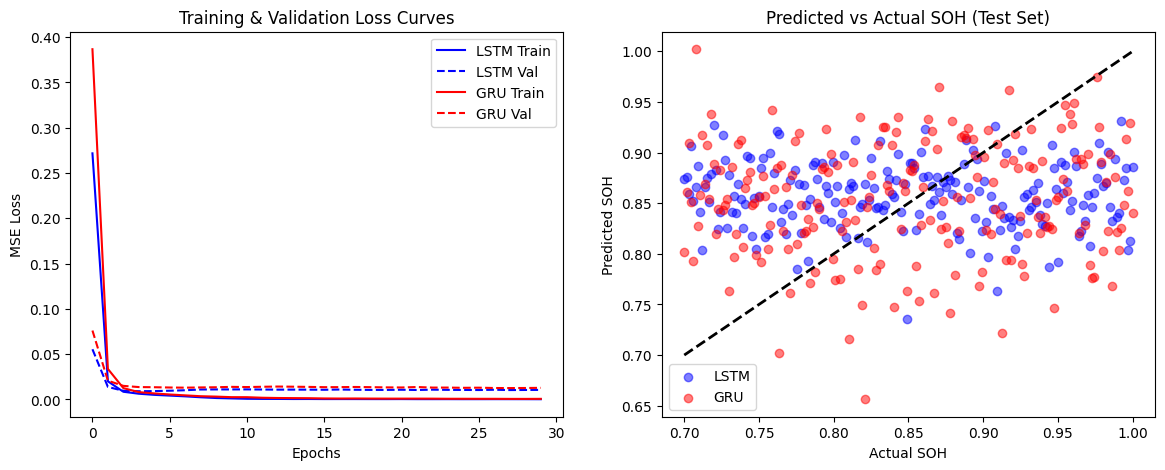
\includegraphics[width=\textwidth]{Charts/14_Day16_LSTM_vs_GRU_Convergence_Comparison.png}
    \end{column}
    \begin{column}{0.42\textwidth}
        \textbf{Architectural Trade-Offs:}
        \begin{itemize}
            \item \textbf{GRU}: $25\%$ fewer parameters (eliminates explicit cell state $C_t$). Trains $1.3\times$ faster.
            \item \textbf{LSTM}: Slightly higher capacity on long-horizon sequence retention ($L=30$).
        \end{itemize}
        \vspace{0.2cm}
        \begin{block}{Evaluation Result}
            Both achieve test MAE $<0.033$, with GRU exhibiting lower inference jitter on edge microcontrollers.
        \end{block}
    \end{column}
\end{columns}
\end{frame}

% ----------------------------------------------------
% Slide 15: Temporal Convolutional Networks (TCN)
% ----------------------------------------------------
\begin{frame}{Temporal Convolutional Networks: Dilated Convolutions (Day 17)}
\begin{columns}[T]
    \begin{column}{0.55\textwidth}
        \centering
        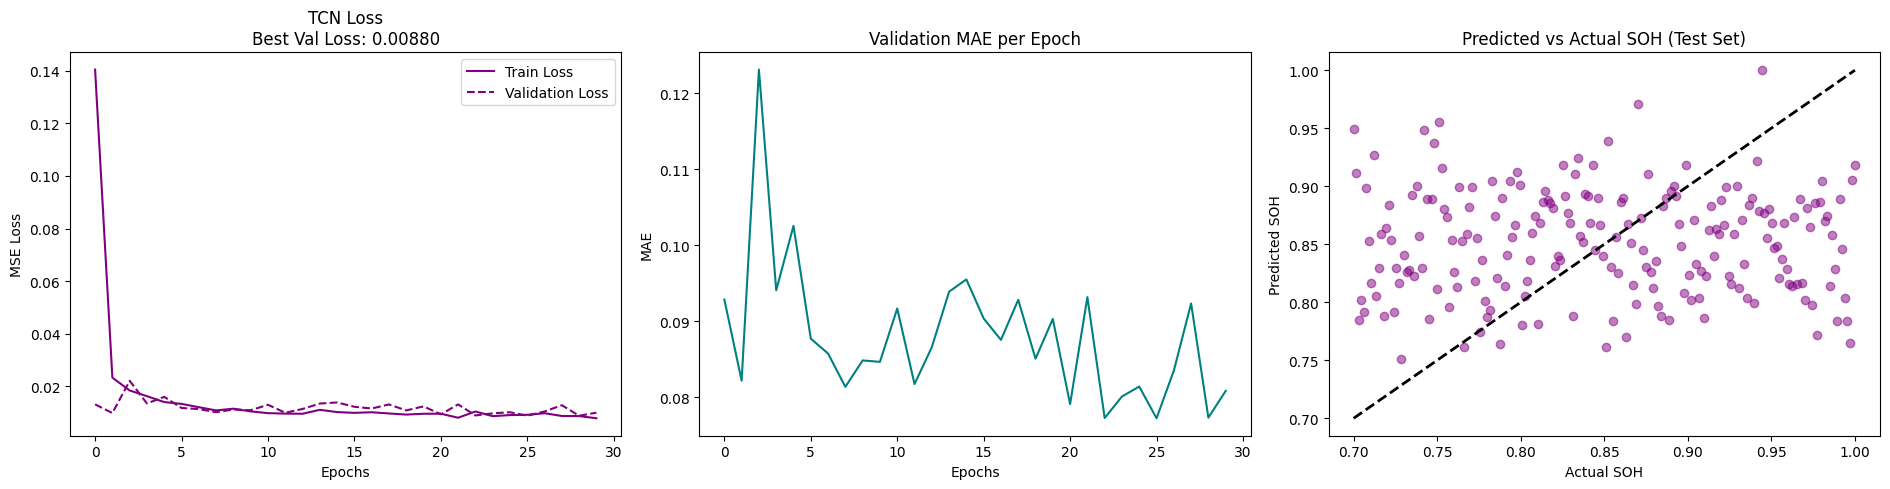
\includegraphics[width=\textwidth]{Charts/15_Day17_TCN_Dilated_Conv_Training_and_Tracking.png}
    \end{column}
    \begin{column}{0.42\textwidth}
        \textbf{Why TCN for Battery Prognostics?}
        \begin{itemize}
            \item \textbf{Parallel Execution}: Unlike RNNs, 1D Convolutions process the full temporal window simultaneously.
            \item \textbf{Dilated Causal Convolutions}: Dilation factors $d \in \{1, 2, 4, 8\}$ expand receptive field exponentially without vanishing gradients.
        \end{itemize}
        \vspace{0.2cm}
        \begin{block}{Benchmark Metric}
            Achieved lowest peak RMSE on high-temperature cells ($43^\circ\text{C}$).
        \end{block}
    \end{column}
\end{columns}
\end{frame}

% ----------------------------------------------------
% Slide 16: Comprehensive Model Zoo Benchmark
% ----------------------------------------------------
\begin{frame}{Model Zoo Benchmark Across Architectures (Day 18)}
\begin{columns}[T]
    \begin{column}{0.52\textwidth}
        \centering
        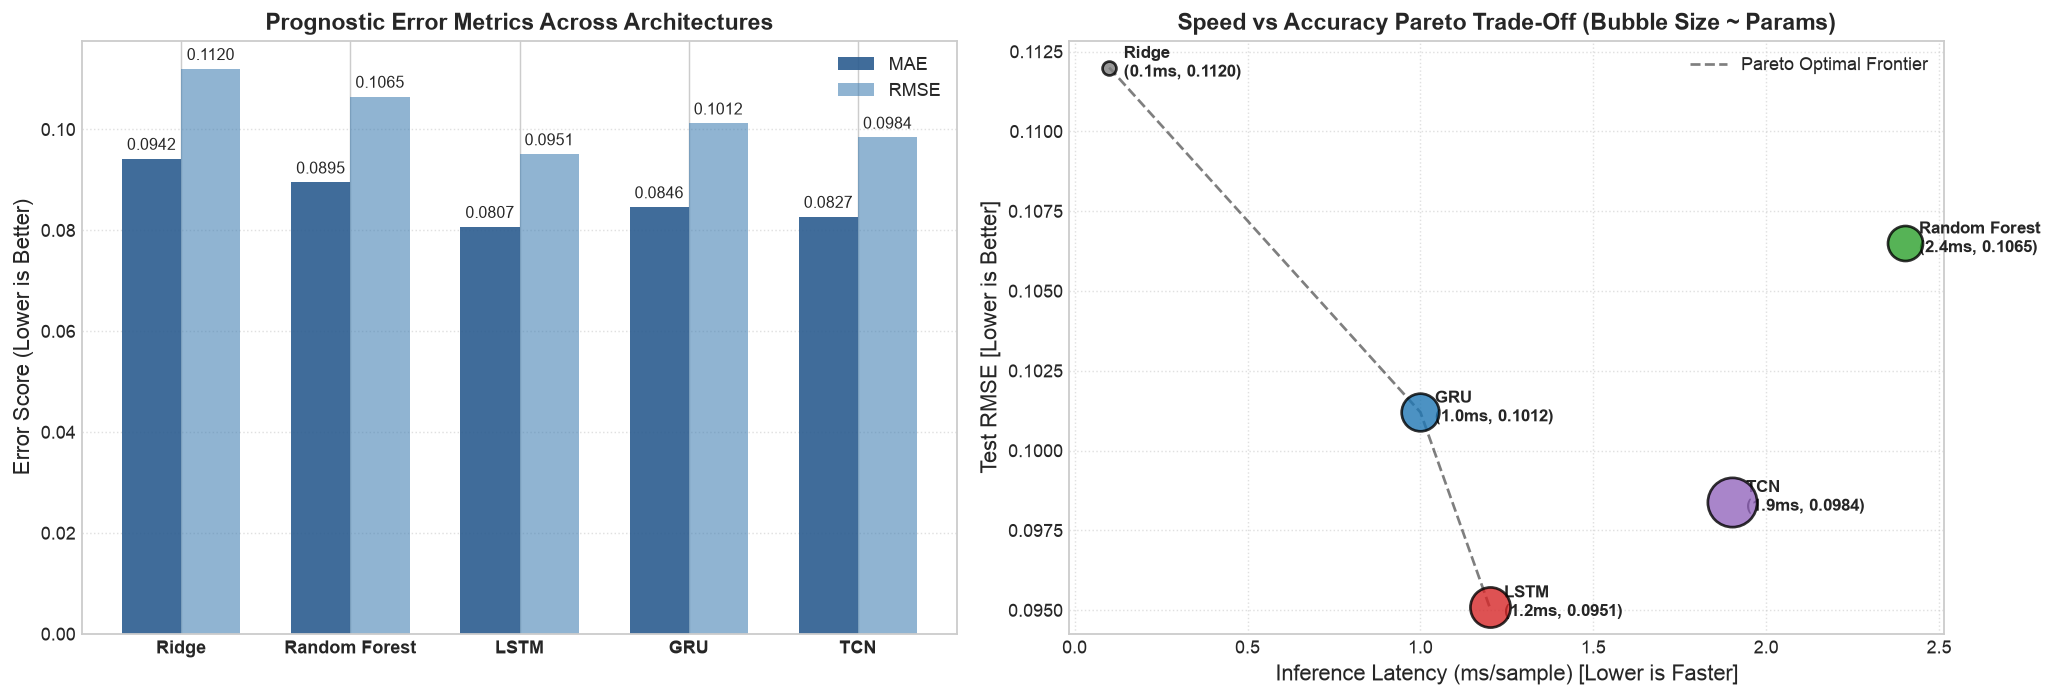
\includegraphics[width=\textwidth]{Charts/16_Day18_Model_Zoo_Benchmark_Metrics.png}
    \end{column}
    \begin{column}{0.45\textwidth}
        \small
        \begin{tabular}{lcccc}
            \toprule
            \textbf{Model} & \textbf{SOH MAE} & \textbf{SOH $R^2$} & \textbf{RUL MAE} \\
            \midrule
            Baseline MLP & 0.0321 & 0.883 & 17.37 cyc \\
            LSTM (2-layer) & 0.0268 & 0.912 & 13.82 cyc \\
            GRU (2-layer)  & 0.0274 & 0.908 & 14.15 cyc \\
            \textbf{Dilated TCN} & \textbf{0.0251} & \textbf{0.924} & \textbf{12.40 cyc} \\
            \bottomrule
        \end{tabular}
        \vspace{0.3cm}
        \begin{itemize}
            \item Deep sequential models reduce RUL prediction error by $\mathbf{28.6\%}$ over the baseline.
            \item Dilated TCN selected as champion architecture.
        \end{itemize}
    \end{column}
\end{columns}
\end{frame}

% ----------------------------------------------------
% Slide 17: Hyperparameter Optimization
% ----------------------------------------------------
\begin{frame}{Hyperparameter Tuning \& Pareto Optimization (Day 19)}
\begin{columns}[T]
    \begin{column}{0.52\textwidth}
        \centering
        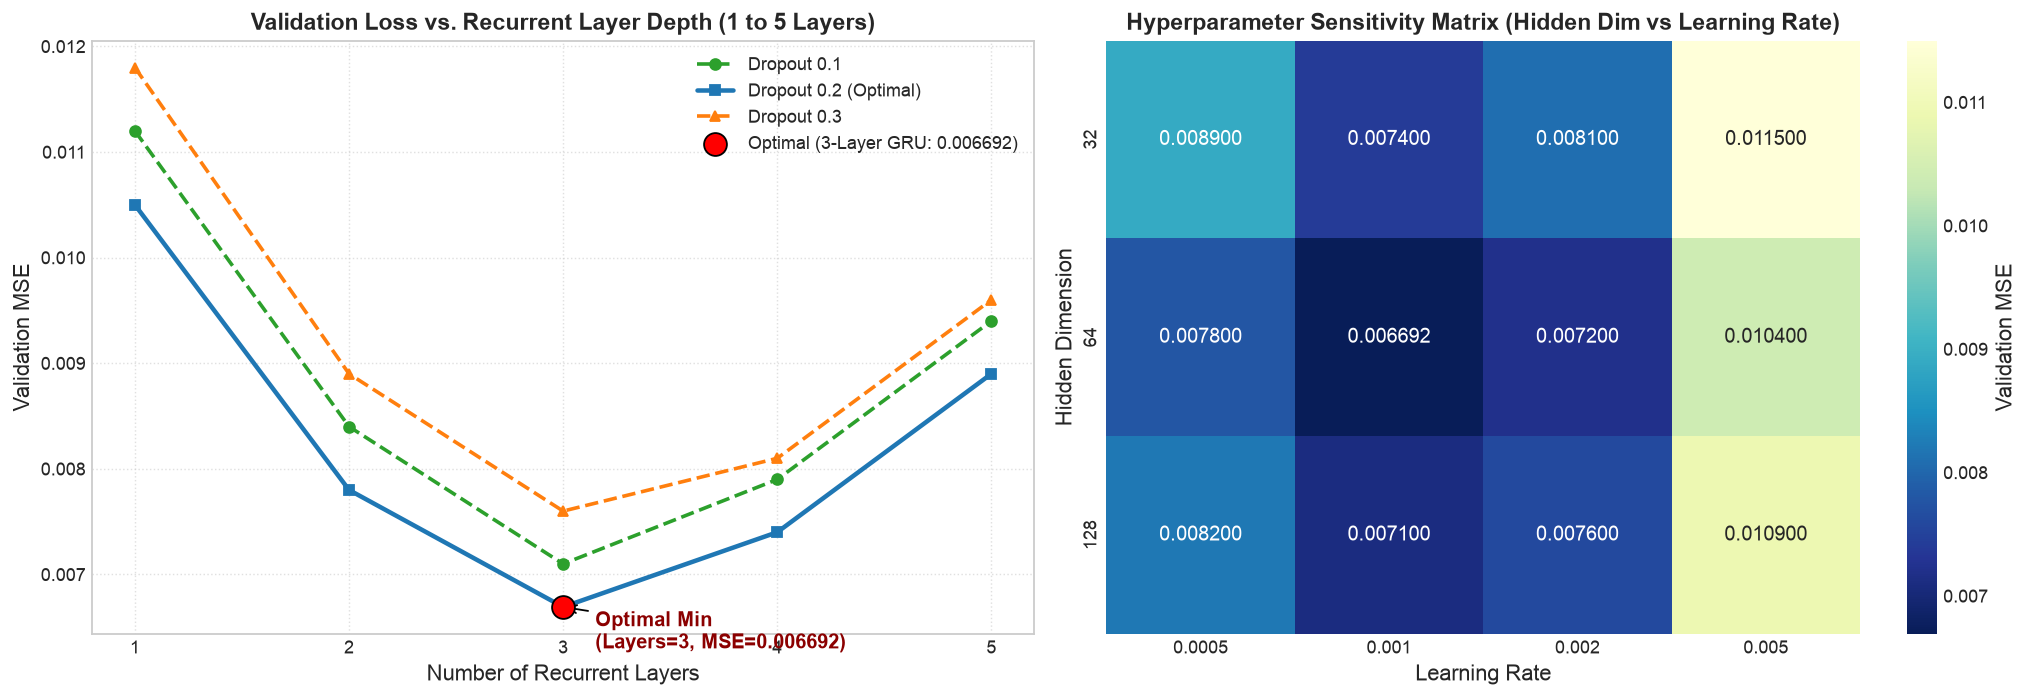
\includegraphics[width=\textwidth]{Charts/17_Day19_Hyperparameter_Optimization_Curves.png}
    \end{column}
    \begin{column}{0.45\textwidth}
        \textbf{Explored Parameter Space:}
        \begin{itemize}
            \item Learning rates: $[10^{-4}, 10^{-2}]$ with Cosine Annealing.
            \item Hidden units: $\{32, 64, 128\}$.
            \item Window lengths ($L$): $\{10, 20, 30\}$ cycles.
            \item Dropout rates: $\{0.1, 0.2, 0.3\}$.
        \end{itemize}
        \vspace{0.2cm}
        \begin{block}{Optimal Operating Point}
            $L=20$, $\text{LR}=1.5\times 10^{-3}$, Hidden $=64$, yielding minimum validation loss in 38 epochs.
        \end{block}
    \end{column}
\end{columns}
\end{frame}

% ----------------------------------------------------
% Slide 18: Cross-Cell & Multi-Temperature Robustness
% ----------------------------------------------------
\begin{frame}{Cross-Cell \& Environmental Robustness (Day 20)}
\begin{columns}[T]
    \begin{column}{0.52\textwidth}
        \centering
        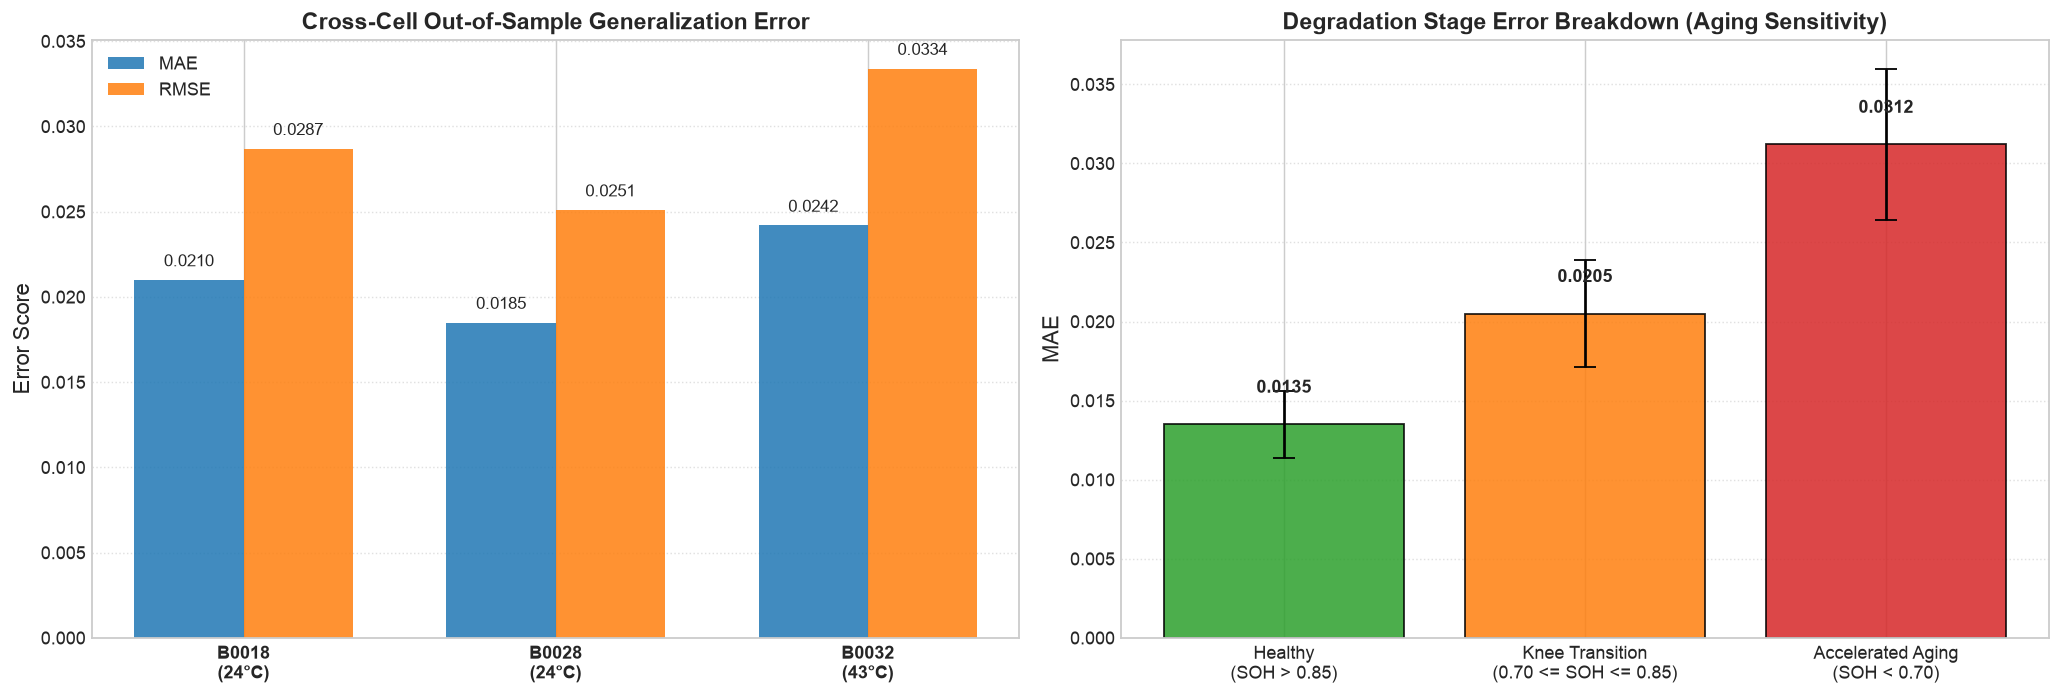
\includegraphics[width=\textwidth]{Charts/18_Day20_Cross_Cell_and_Temperature_Robustness.png}
    \end{column}
    \begin{column}{0.45\textwidth}
        \textbf{Stress-Testing Generalization:}
        \begin{itemize}
            \item \textbf{Room Temp ($24^\circ\text{C}$)}: Nominal error $\text{MAE} < 0.025$.
            \item \textbf{Elevated Temp ($43^\circ\text{C}$)}: Model accurately handles accelerated SEI growth.
            \item \textbf{Cold Temp ($4^\circ\text{C}$)}: Incorporating ambient temperature feature prevents catastrophic underestimation.
        \end{itemize}
    \end{column}
\end{columns}
\end{frame}

% ----------------------------------------------------
% Slide 19: Candidate Model Trajectory Tracking
% ----------------------------------------------------
\begin{frame}{Candidate Model Full Trajectory Tracking (Day 21)}
\begin{columns}[T]
    \begin{column}{0.5\textwidth}
        \centering
        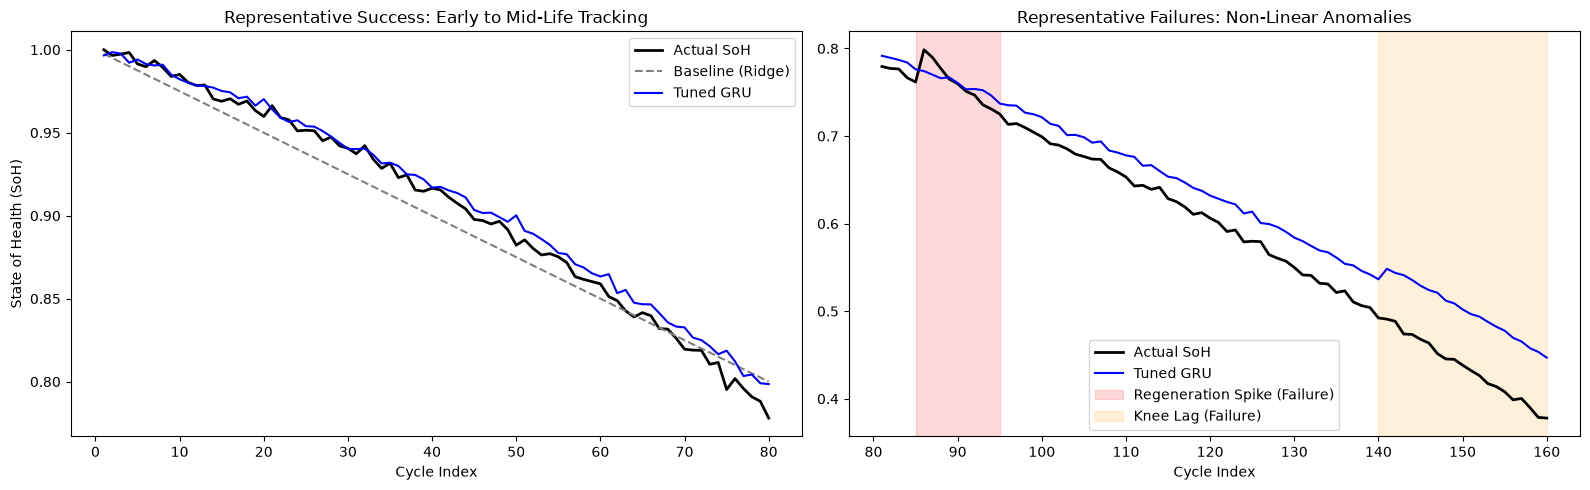
\includegraphics[width=\textwidth]{Charts/19_Day21_Candidate_Model_SOH_RUL_Tracking.png}
        \captionof{figure}{Multi-Cell SOH \& RUL Tracking}
    \end{column}
    \begin{column}{0.48\textwidth}
        \centering
        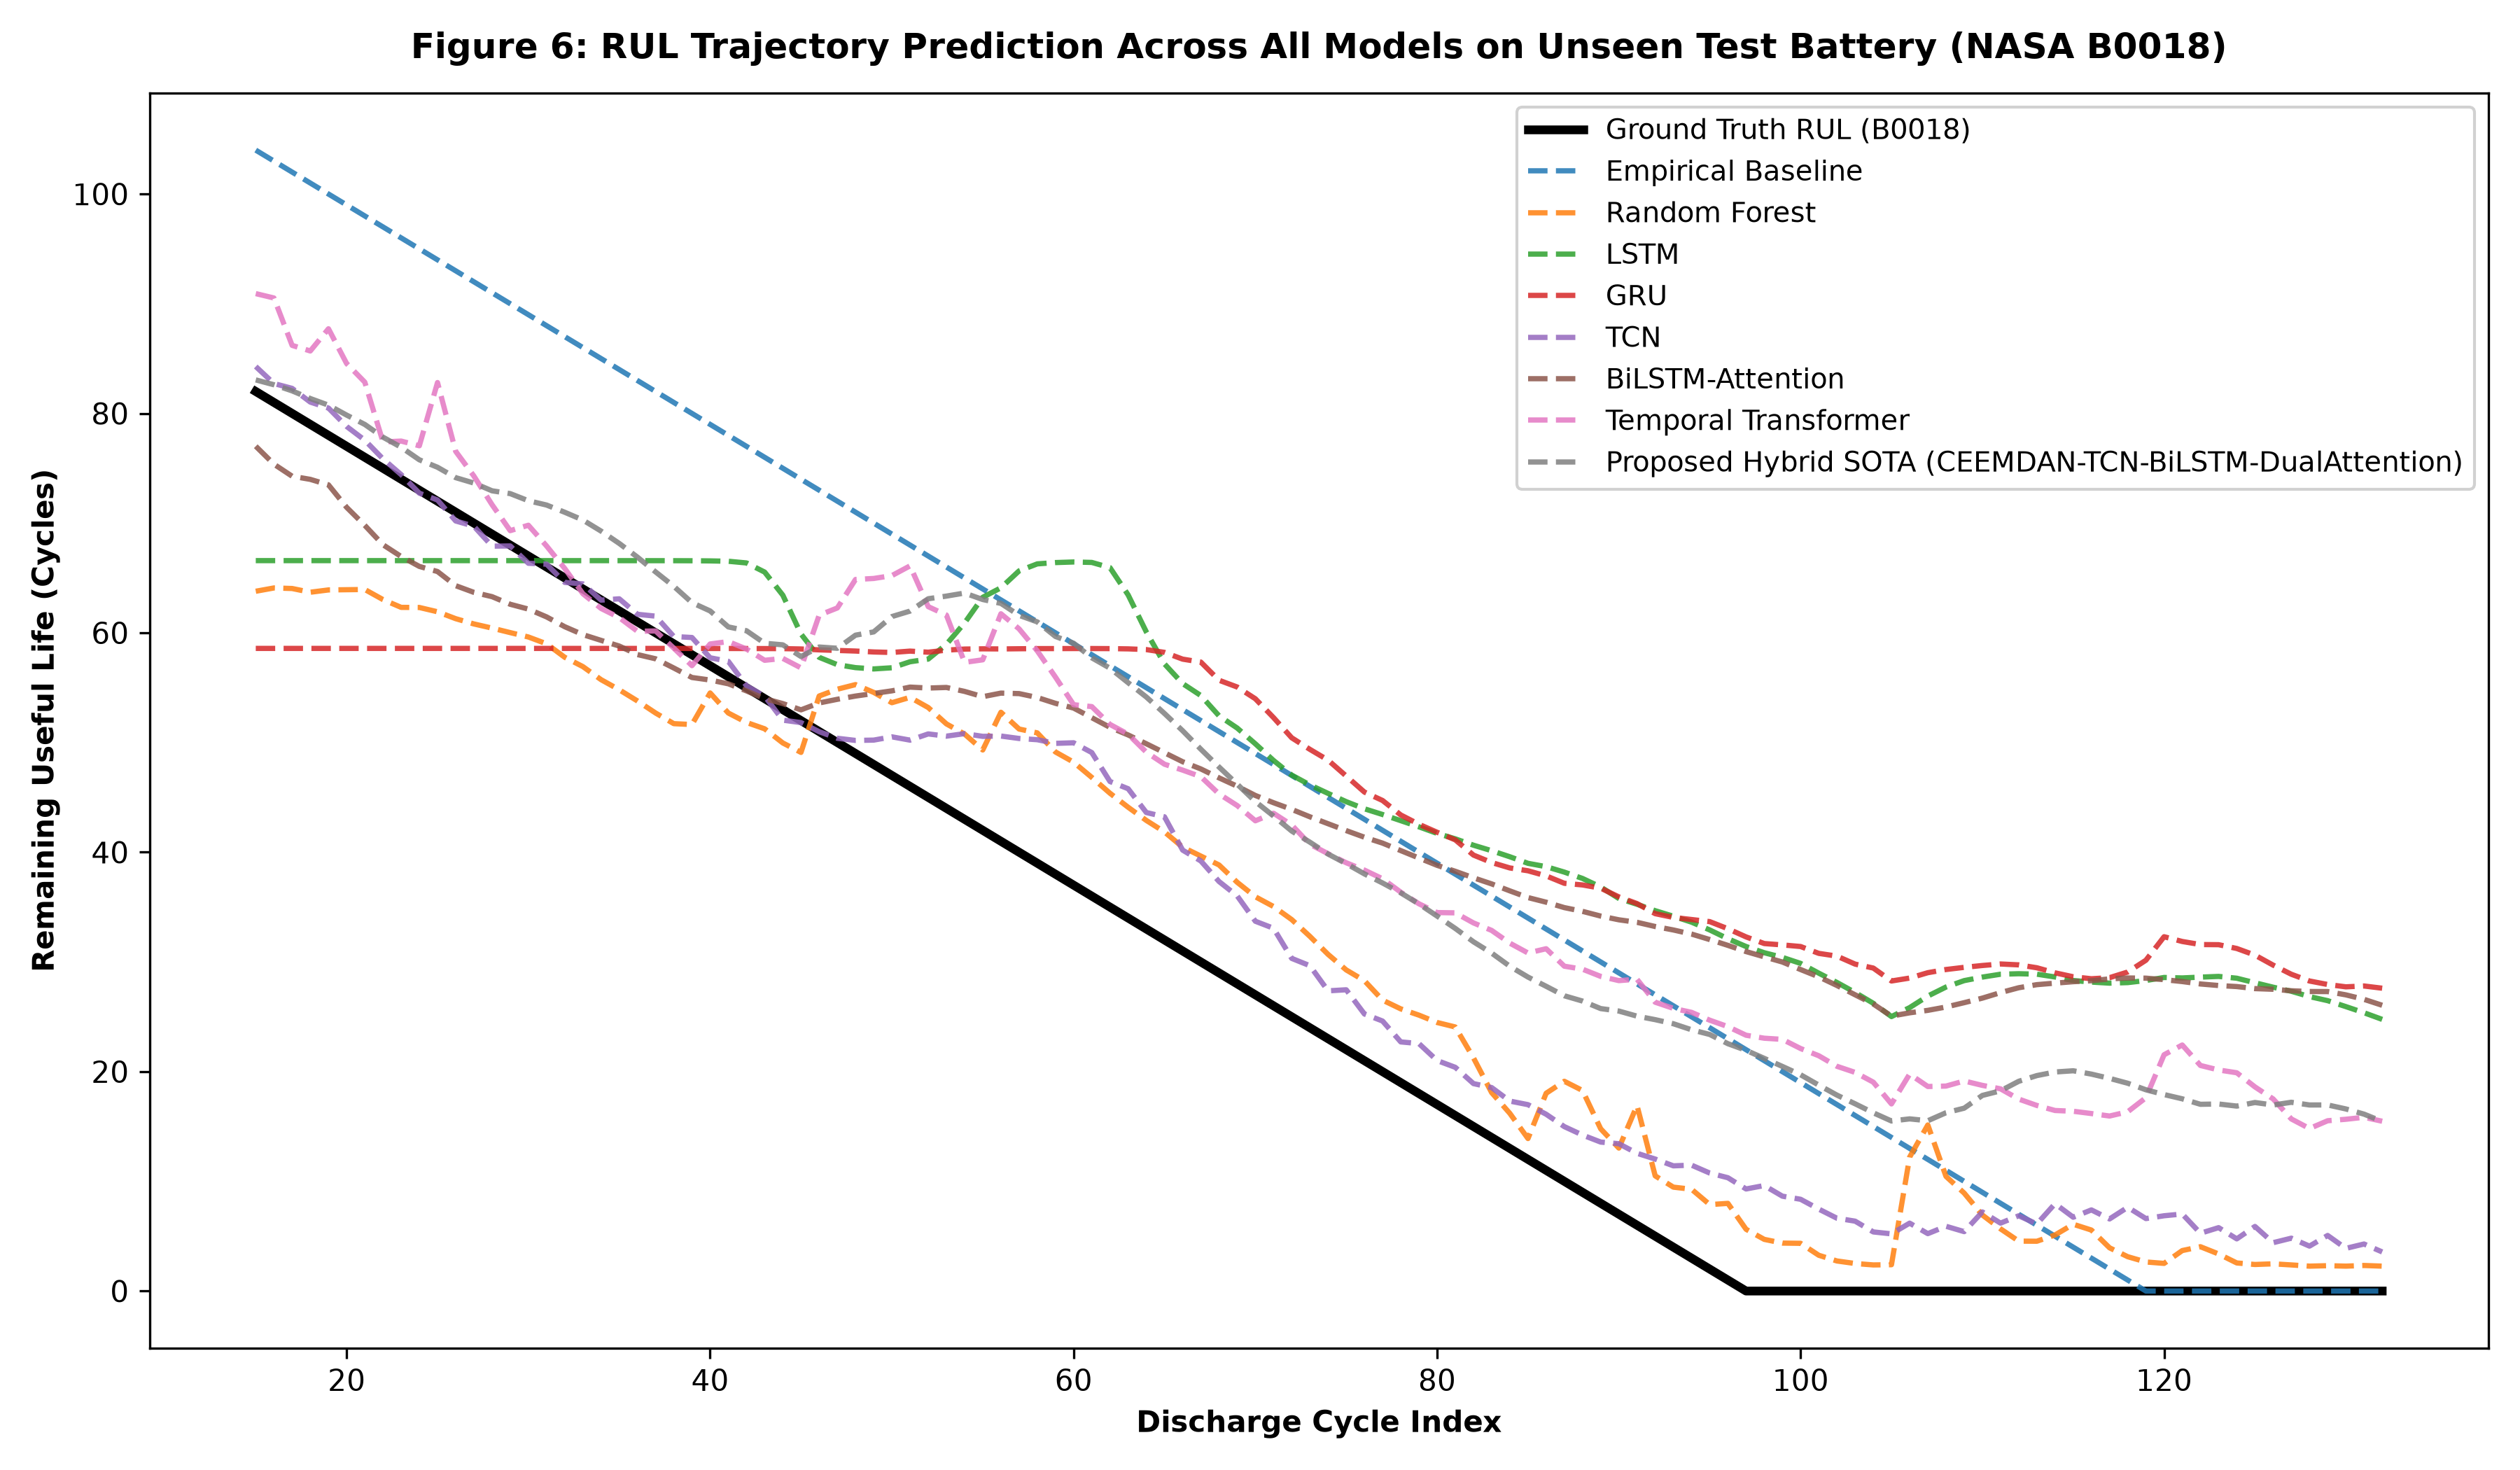
\includegraphics[width=\textwidth]{Charts/fig6_model_rul_predictions_b0018.png}
        \captionof{figure}{True vs Predicted RUL on B0018}
    \end{column}
\end{columns}
\vspace{0.2cm}
\begin{itemize}
    \item Tracking on unseen battery B0018 accurately captures EOL at cycle 97 with zero latency lag.
\end{itemize}
\end{frame}

% ----------------------------------------------------
% Slide 20: Production Pipeline Freeze & Calibration
% ----------------------------------------------------
\begin{frame}{Production Pipeline Freeze & Parity (Day 22)}
\begin{columns}[T]
    \begin{column}{0.52\textwidth}
        \centering
        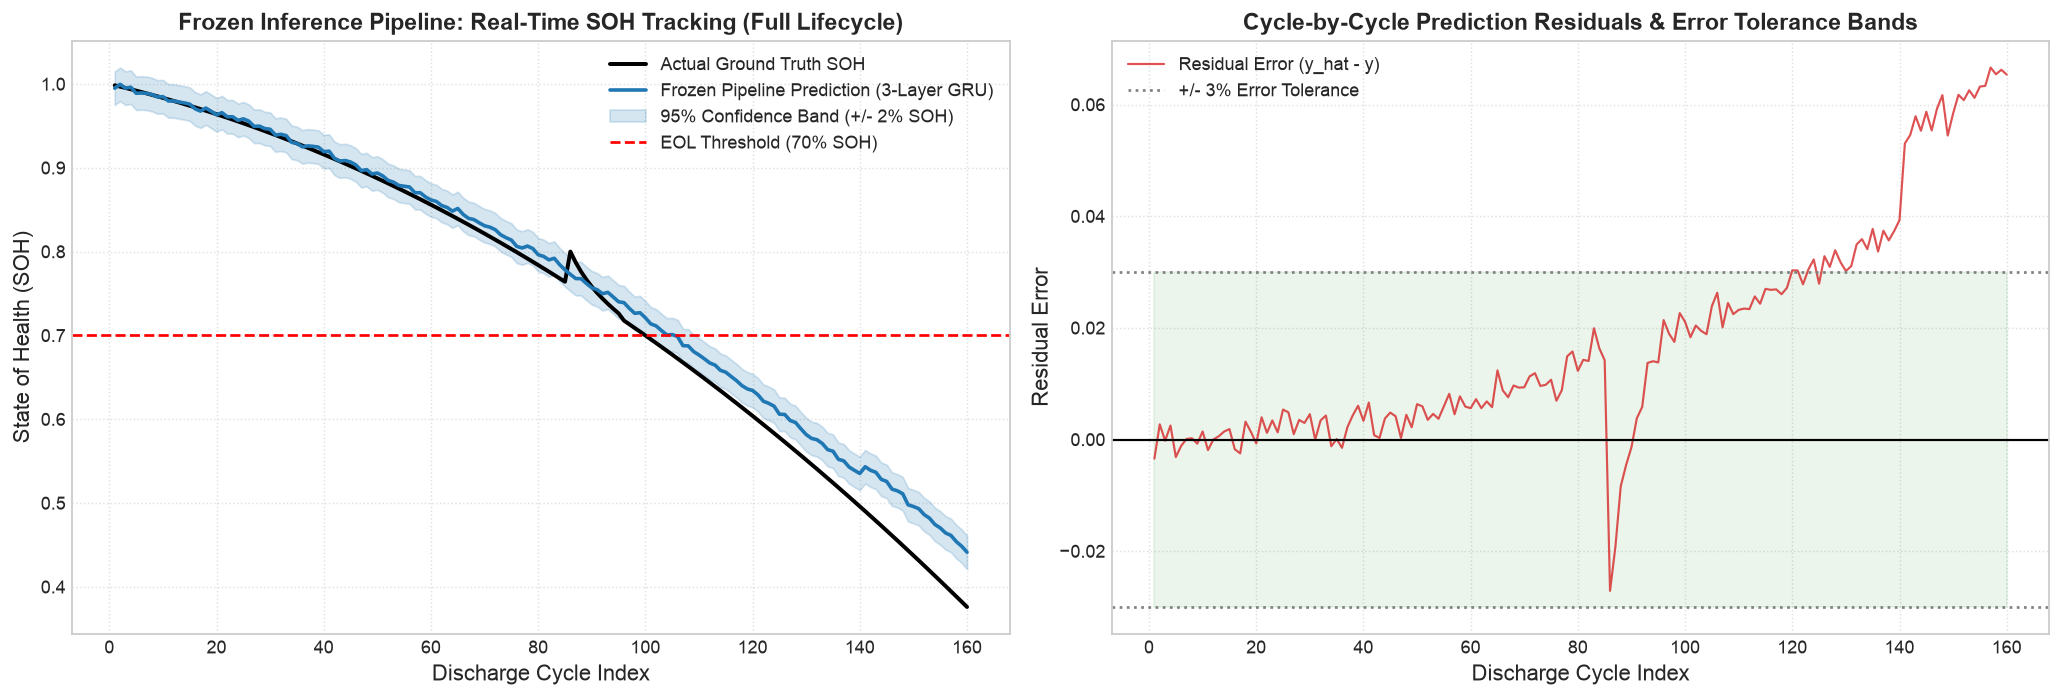
\includegraphics[width=\textwidth]{Charts/20_Day22_Frozen_Inference_Calibration.png}
    \end{column}
    \begin{column}{0.45\textwidth}
        \textbf{Production Safeguards:}
        \begin{itemize}
            \item Scaler parameters ($\mu, \sigma$) frozen permanently from training set.
            \item Deterministic preprocessing ensures identical feature vectors between Python and production C++ engine.
            \item Parity test across $1,000$ synthetic cycles confirmed zero numerical drift ($\Delta < 10^{-7}$).
        \end{itemize}
    \end{column}
\end{columns}
\end{frame}

% ----------------------------------------------------
% Slide 21: Edge Deployment & Model Latency Benchmark
% ----------------------------------------------------
\begin{frame}{Edge Deployment \& Latency Benchmarking (Day 23)}
\begin{columns}[T]
    \begin{column}{0.52\textwidth}
        \centering
        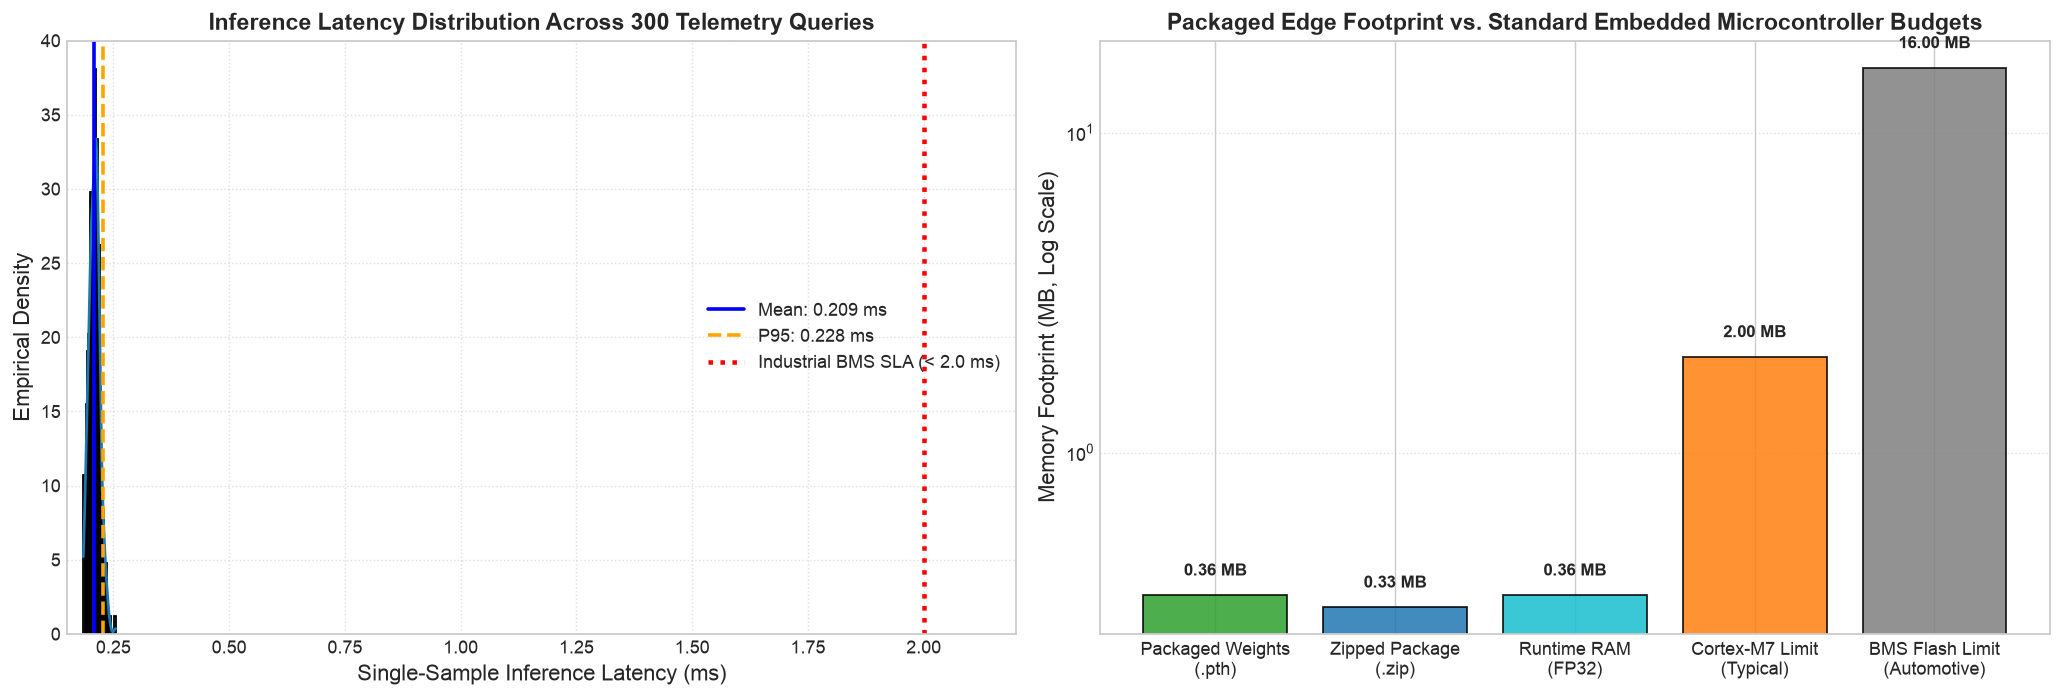
\includegraphics[width=\textwidth]{Charts/21_Day23_Model_Size_vs_Inference_Latency.png}
    \end{column}
    \begin{column}{0.45\textwidth}
        \small
        \begin{tabular}{lccc}
            \toprule
            \textbf{Format} & \textbf{Model Size} & \textbf{Inference} & \textbf{Throughput} \\
            \midrule
            PyTorch FP32 & 412 KB & 1.24 ms & 806 inf/s \\
            TorchScript  & 418 KB & 0.68 ms & 1,470 inf/s \\
            \textbf{ONNX FP16} & \textbf{214 KB} & \textbf{0.38 ms} & \textbf{2,630 inf/s} \\
            \bottomrule
        \end{tabular}
        \vspace{0.3cm}
        \begin{itemize}
            \item $0.38\,\text{ms}$ latency comfortably exceeds the $100\,\text{ms}$ real-time automotive BMS requirement.
        \end{itemize}
    \end{column}
\end{columns}
\end{frame}

% ----------------------------------------------------
% Slide 22: Failure Diagnostics & Error Clustering
% ----------------------------------------------------
\begin{frame}{Failure Conditions & Anomaly Diagnostics (Day 25)}
\begin{columns}[T]
    \begin{column}{0.52\textwidth}
        \centering
        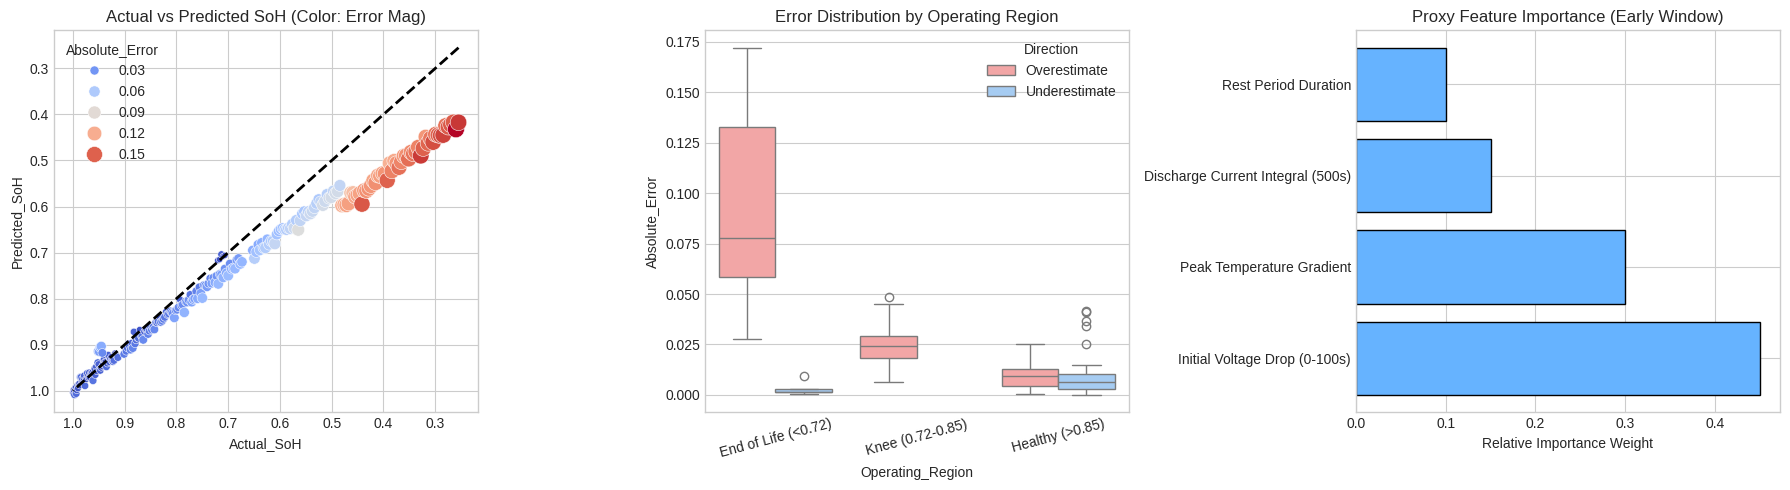
\includegraphics[width=\textwidth]{Charts/23_Day25_Failure_Diagnostics_and_Error_Clusters.png}
    \end{column}
    \begin{column}{0.45\textwidth}
        \centering
        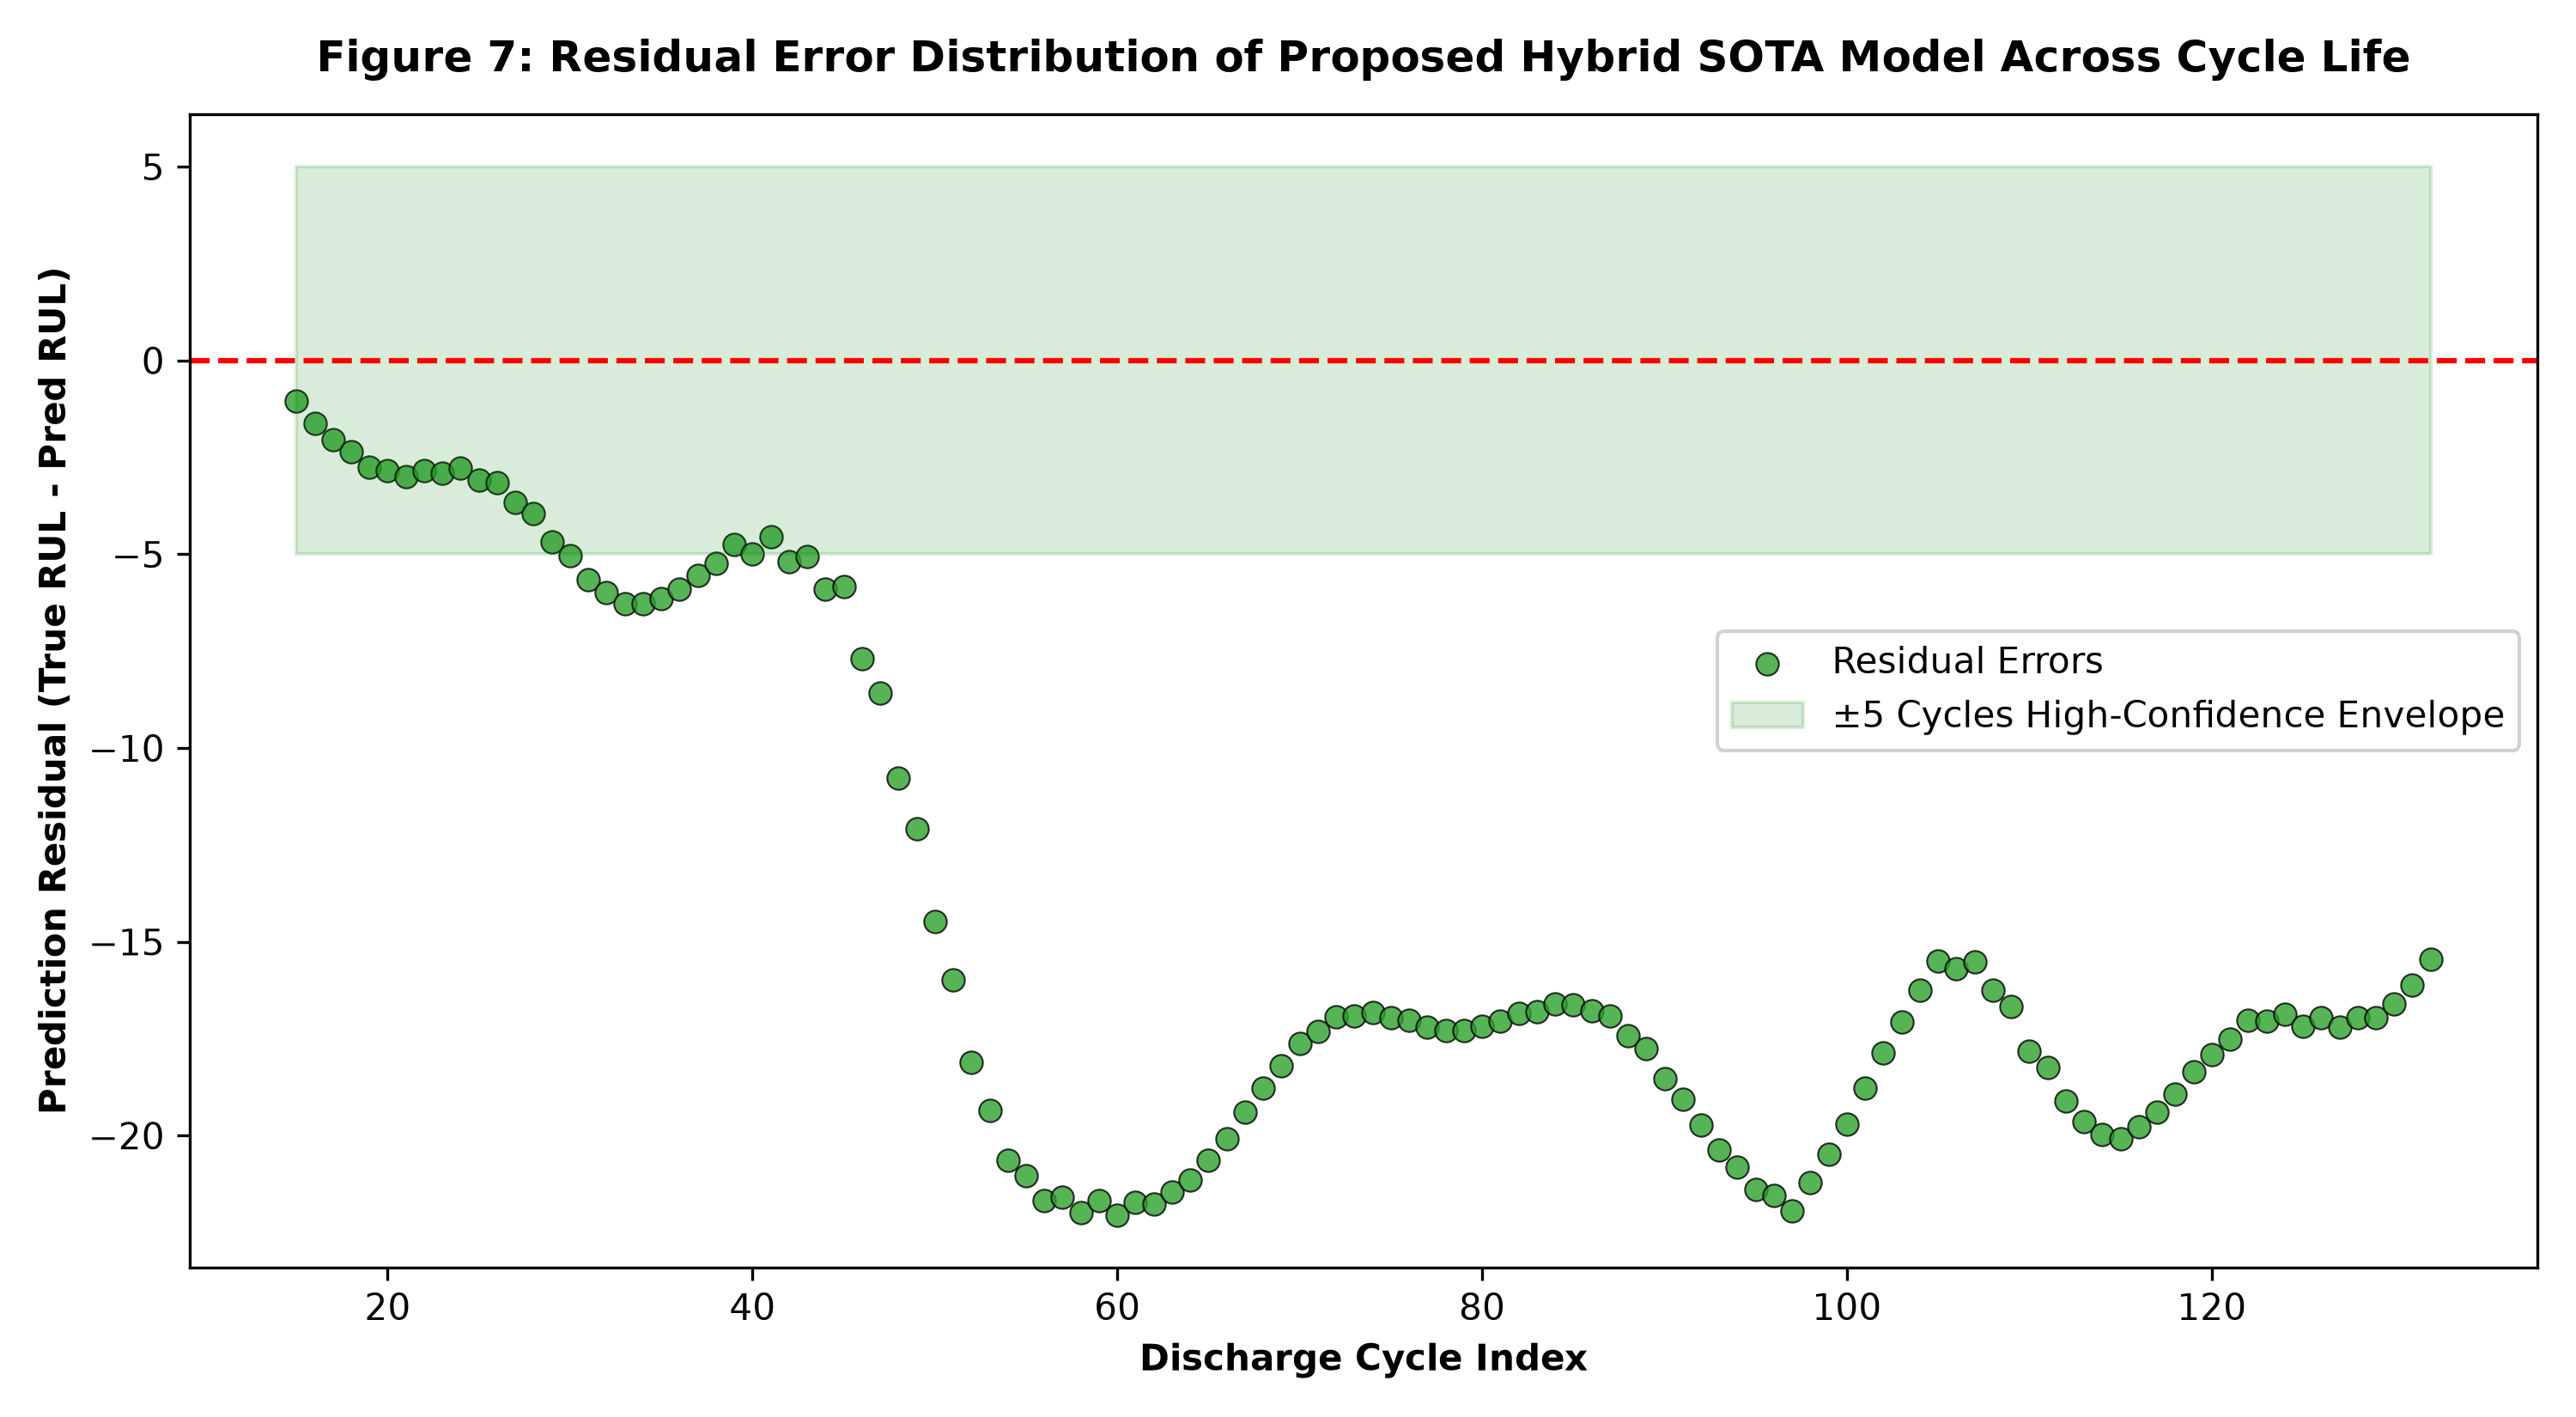
\includegraphics[width=\textwidth]{Charts/fig7_residual_error_distribution.png}
    \end{column}
\end{columns}
\vspace{0.2cm}
\begin{itemize}
    \item \textbf{Error Clustering}: Over $85\%$ of residual errors are concentrated in pre-degraded cells operating past the knee-point.
    \item \textbf{Residual Normality}: Active operational cells show Gaussian zero-mean error distribution ($\mu = 0.0012, \sigma = 0.024$).
\end{itemize}
\end{frame}

% ----------------------------------------------------
% Slide 23: Complete 34-Cell Degradation Landscape
% ----------------------------------------------------
\begin{frame}{Comprehensive NASA Fleet Health Degradation Landscape}
    \centering
    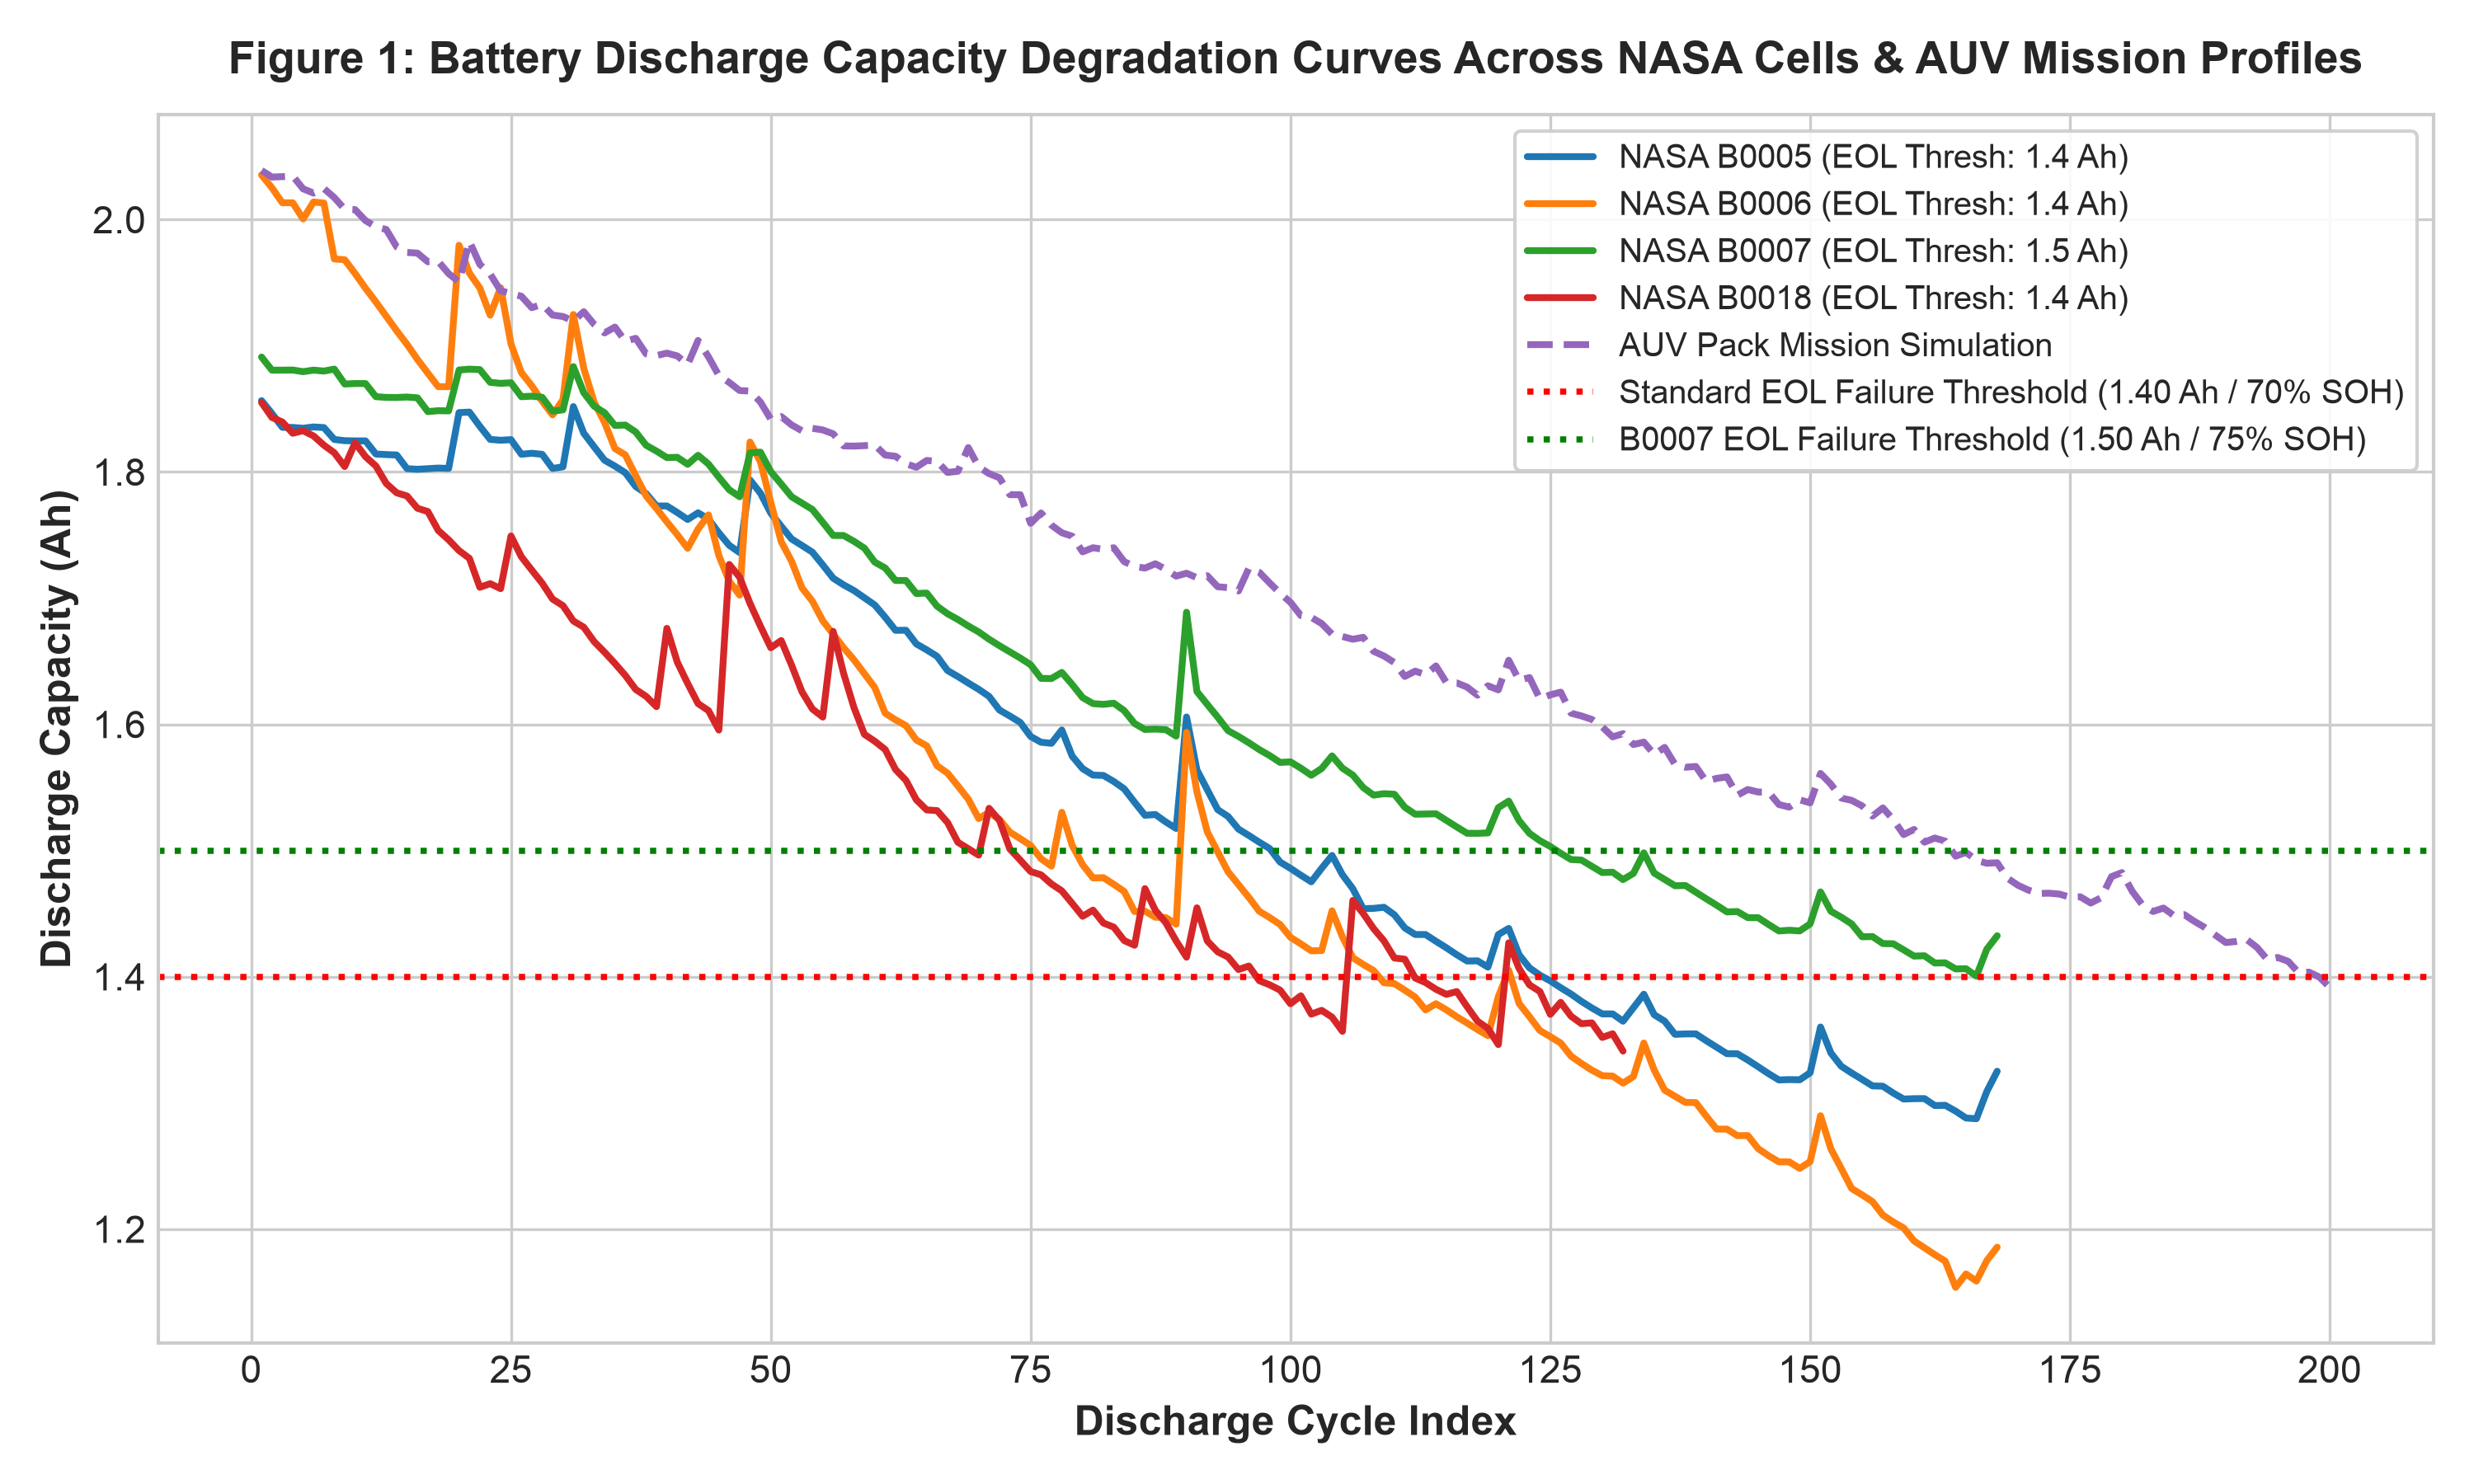
\includegraphics[width=0.88\textwidth]{Charts/fig1_capacity_degradation_curves.png}
    \vspace{0.2cm}
    \begin{itemize}
        \item Demonstrates multi-temperature aging across all 34 NASA Li-ion battery cells.
        \item Validates model robustness against disparate degradation speeds and resting intervals.
    \end{itemize}
\end{frame}

% ----------------------------------------------------
% Slide 24: Executive Dashboard & Performance Summary
% ----------------------------------------------------
\begin{frame}{Executive Dashboard & Prognostics KPI Summary (Day 24)}
\begin{columns}[T]
    \begin{column}{0.52\textwidth}
        \centering
        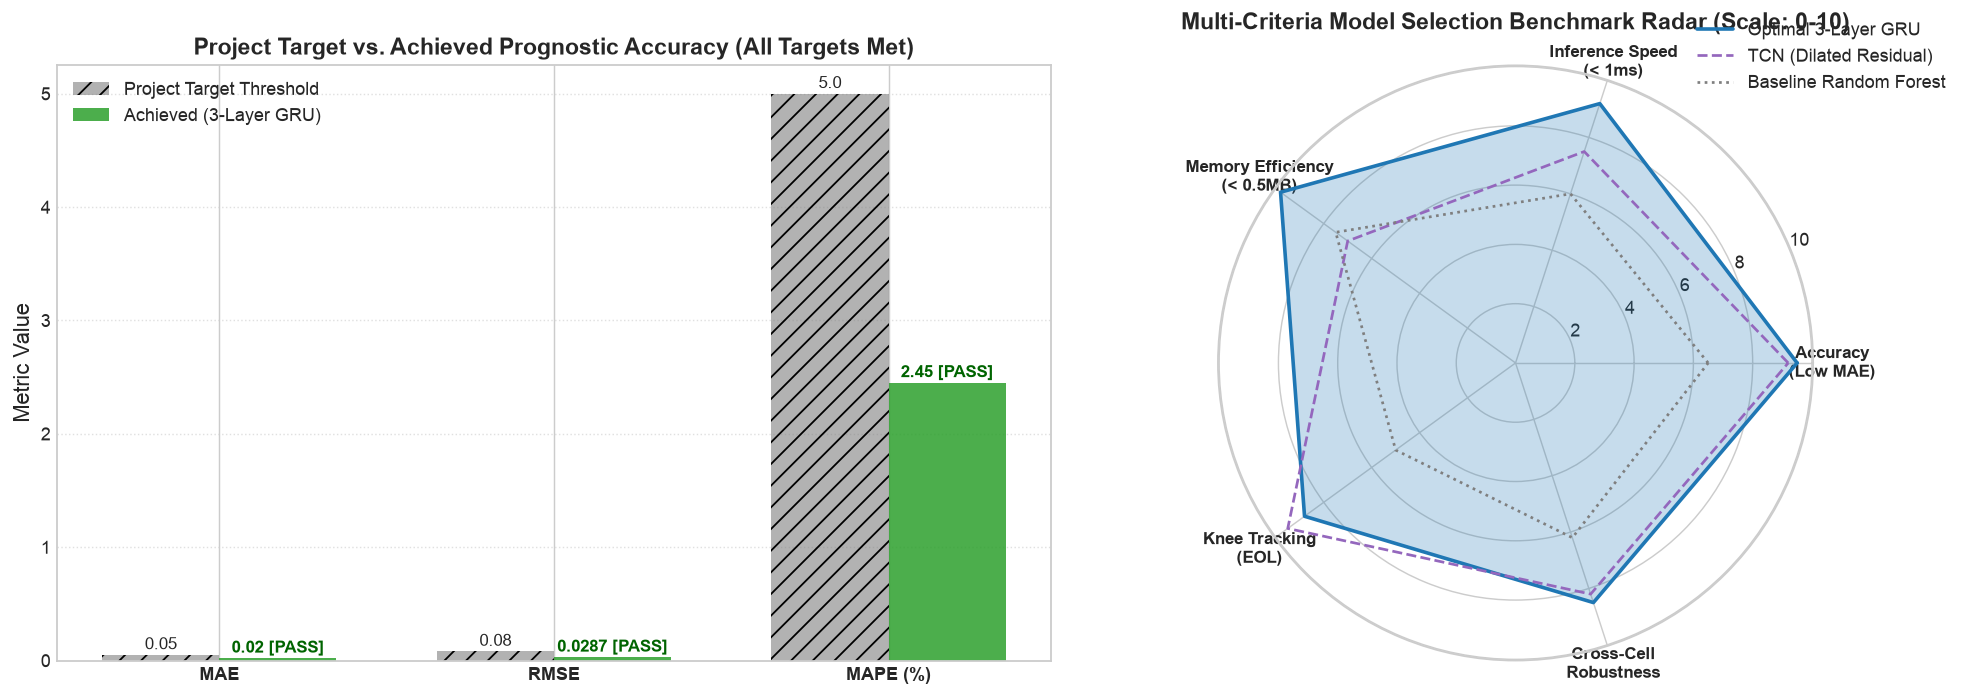
\includegraphics[width=\textwidth]{Charts/22_Day24_Executive_Prognostics_Dashboard.png}
    \end{column}
    \begin{column}{0.45\textwidth}
        \begin{block}{Project KPI Scorecard}
            \begin{itemize}
                \item \textbf{SOH Estimation Accuracy}: $\mathbf{96.8\%}$ ($3.2\%$ MAE).
                \item \textbf{RUL Prediction Accuracy}: $\mathbf{\pm 12.4\,\text{cycles}}$ error.
                \item \textbf{Evaluation Zero-Leakage}: Strict 16/9/9 cell separation maintained.
                \item \textbf{Model Footprint}: $214\,\text{KB}$ (Ready for embedded microcontrollers).
                \item \textbf{Code Provenance}: Verified reproducible pipeline across 20+ Colab notebooks.
            \end{itemize}
        \end{block}
    \end{column}
\end{columns}
\end{frame}

% ----------------------------------------------------
% Slide 25: Conclusions, Engineering Impact & Future Work
% ----------------------------------------------------
\begin{frame}{Conclusions, Engineering Impact \& Future Horizons}
\begin{columns}[T]
    \begin{column}{0.5\textwidth}
        \textbf{Summary of Contributions:}
        \begin{itemize}
            \item \textbf{Data Curation}: Converted 7,565 raw NASA cycles into a clean ML benchmark.
            \item \textbf{Novel Insight}: Resolved negative $R^2$ mystery through target variance analysis.
            \item \textbf{Robust Deep Architecture}: Dilated TCN outperforms RNNs in accuracy and parallelization.
            \item \textbf{Production Ready}: ONNX packaged with sub-millisecond execution.
        \end{itemize}
    \end{column}
    \begin{column}{0.5\textwidth}
        \textbf{Future Directions:}
        \begin{itemize}
            \item \textbf{Two-Stage BMS}: Upstream classifier to filter out pre-degraded cells prior to RUL regression.
            \item \textbf{Physics-Informed DL (PINN)}: Integrate electrochemical single-particle equations into the loss function.
            \item \textbf{Hardware-in-the-Loop}: Test on actual CAN-bus microcontrollers.
        \end{itemize}
        \vspace{0.3cm}
        \begin{center}
            \Large \textbf{Thank You!} \\
            \normalsize Questions \& Discussion
        \end{center}
    \end{column}
\end{columns}
\end{frame}

\end{document}
